% !TeX root = RJwrapper.tex
\title{\pkg{MSmix}: An \textsf{R} Package for clustering partial rankings via mixtures of Mallows Models with Spearman distance}
\author{Marta Crispino$^*$, Cristina Mollica$^*$, Lucia Modugno\\\
$^*$ jointly first authors}

\maketitle

\abstract{
  \pkg{MSmix} is a recently developed \textsf{R} package implementing maximum likelihood estimation of finite mixtures of Mallows models with Spearman distance for full and partial rankings. The package is designed to implement computationally tractable estimation routines, with the ability to handle arbitrary forms of partial rankings and a large number of items. The frequentist estimation task is accomplished via Expectation-Maximization algorithms, integrating data augmentation strategies to recover the unobserved heterogeneity and the missing ranks. The package also provides functionalities for uncertainty quantification of the parameter estimates, via diverse bootstrap methods and asymptotic confidence intervals.
  Generic methods for S3 class objects are constructed for more effectively managing the output of the main routines.
  The usefulness of the package and its computational performance compared with competing software is illustrated via applications to both simulated and original real ranking datasets.
}

\section[Intro]{Introduction}
Ranking data play a pivotal role in numerous research and practical domains, where the focus is on comparing and ordering a set of $n$ items according to personal preferences or other relevant criteria. From market surveys to sports competitions, from academic assessments to online recommendation systems, rankings are ubiquitous in modern society to capture human choice behaviors or, more generally, ordinal comparison processes in various contexts.

{
Ranking data analysis has attracted significant attention, as evidenced by the extensive literature on the subject \citep[see][for fundamental reviews]{critchlow91probability, Marden1995} and by the development of a broad spectrum of probabilistic models designed to capture meaningful choice patterns and quantify estimation uncertainty.
Traditionally, four main classes of parametric models have been identified, each representing a distinct ranking generative process. The first category, order statistics models (OSs), is originally attributed to \cite{thurstone27law} and conceptualizes rankings as arising from the ordering of latent item utilities. The second, paired comparison models, is exemplified by the Bradley-Terry model (BT) proposed by \citet{bradley1952rank} and is based on the possibility to decompose a ranking sequence into the corresponding set of pairwise comparisons. The third category, stagewise models, breaks the ranking process into sequential stages and is well represented by the popular Plackett-Luce model (PL) introduced by \cite{Luce1959} and \cite{Plackett1975}. Finally, distance-based models, often referred to as \textit{Mallows models} (MMs), trace their origins to the seminal work by \citet{Mallows1957}.
In this paper, we focus on the last class,
which provides an ideal option for applications where a meaningful consensus ranking can be identified in the sample and, consequently, offers a valuable parametric tool for rank aggregation tasks \citep{Marden1995}. For further insights into probabilistic ranking models and their unique characteristics, that can support the critical choice of suitable parametric families for specific real contexts, the reader is referred to \citet{Liu2019} and \citet{AlvoYu2014}.}

The MM is based on the assumption that a modal consensus ranking of the $n$ items exists in the population, effectively capturing the collective preferences. Under this framework, the likelihood of observing any particular ranking decreases as its distance from the consensus increases.
{While the distance measure in the MM induces distinct probabilistic models, it only needs to satisfy minimal properties. This simplicity offers researchers remarkable flexibility to choose the distance that best fits their scientific context. For example, Kendall and Cayley distances are well suited for sorting problems, Hamming works well in coding theory, and Spearman distance is particularly suitable for applications involving human preferences or social choice \citep{Diaconis1988}.}
Traditionally, the choice of the distance in the MM was mainly driven by computational considerations, specifically the availability of a closed-form expression for the model normalizing constant (or \textit{partition function}). This favored the use of Kendall, Cayley, and Hamming distances, while the Spearman distance has been relatively underexplored due to its perceived intractability, despite its relevance in preference domains. However, \citet{crispino23efficient} recently demonstrated that the Spearman distance is a metric that combines both computational feasibility and interpretability. By leveraging the unique properties of the Spearman distance, and by means of a novel approximation of the model partition function, the authors addressed the critical inferential challenges that historically limited its application. Their approach enabled the development of an efficient strategy to fit the MM with Spearman distance (MMS) for datasets with arbitrary forms of partial rankings. Moreover, they extended the model to finite mixtures, allowing the capture of possible unobserved sample heterogeneity.

{Clustering ranking data to detect and characterize groups with similar preferences has long been a major motivation for extending traditional methods beyond their basic forms. This practical need is reflected in the fact that nearly all \textsf{R} packages dedicated to ranking analysis include clustering methods. From a methodological perspective, the clustering problem has been tackled using both model-based strategies and machine learning approaches. For example, the \pkg{PLMIX} package \citep{mollica2020plmix} fits finite PL mixtures for partial top rankings within the Bayesian framework \citep{mollica2017bayesian}, which notably recovers the maximum likelihood estimation (MLE) described in \cite{gormley2006analysis} as a special case when a noninformative prior is specified. For the same parametric class, the \pkg{PlackettLuce} package \citep{turner2020} implements MLE procedures for generalizations of the PL model that are capable of handling partial and tied rankings, as well as including covariates to achieve model-based partitioning via PL trees.
Concerning OSs, the \pkg{StatRank} package addresses the estimation of finite mixture generalizations from both full and partial rankings through the generalized method of moments \citep{soufiani}.
Additionally, the \textsf{R} package \pkg{Rankcluster} \citep{Rankcluster}, offers an innovative model-based clustering approach through mixtures of Insertion Sort Rank data models \citep{Jacques2014}, which is able to handle partial rankings with arbitrary patterns of incompleteness and, if needed, with multivariate (hierarchical) structures.
An additional contribution to rankings with missing data is provided by the \pkg{prefmod} package \citep{prefmod2012}, which primarily analyzes preference data in the form of paired comparisons, hence also rankings as a by-product, by using the BT and extensions thereof to accommodate ties, subject- and item-specific covariates, as well as partial observations with different censoring forms and missingness processes. However, the extension proposed in \citet{prefmod2012} for clustering heterogeneous data relies on the introduction of non-parametric random-effects models that, in the case of rankings, are implemented only for completely-observed sequences \citep{prefmod.package}.}

{Regarding the availability of software which is more related to our proposal, one can first notice that only a few packages of the Comprehensive R Archive Network (CRAN) implement MMs and generalizations thereof.
}
\pkg{BayesMallows} \citep{BayesMallows} is the unique package adopting the Bayesian perspective to perform inference for the MM and its finite mixture extension.
The flexibility of \pkg{BayesMallows} stands in the wide range of supported distances (including Spearman) and ranked data formats (complete and partial rankings, as well as pairwise comparisons). Moreover, \pkg{BayesMallows} provides estimation uncertainty by building posterior credible sets for the model parameters. Although Bayesian inference of ranking data is effectively addressed, the \textsf{R} packages adopting the frequentist perspective provide users with less flexibility and computational performance. For example, \pkg{pmr} \citep{pmr_R} performs MLE of several ranking models, including the MM with Kendall, Footrule, and Spearman distances.
However, despite the variety of parametric distributions, \pkg{pmr} does not handle partial rankings nor mixtures.
Additionally, the estimation routines require the enumeration of all $n!$ permutations for the global search of the consensus ranking MLE and the naïve computation of the partition function, implying that the analysis of ranking datasets with $n\geq 12$ items is unfeasible.
The \pkg{rankdist} package \citep{rankdist} fits mixtures of MMs with various basic and weighted metrics \citep{lee2012mixtures}, including the Spearman, on a sample of either full or top-$k$ partial rankings. While the implementation for the Kendall distance is highly efficient, it shares similar drawbacks with
\pkg{pmr}, since the partition function of the MMS is computed by summing over all $n!$ permutations, and the MLE of the consensus ranking is obtained through a time-consuming
local search.
As a result, the procedures can be highly demanding, especially in mixture model applications. Moreover, the package does not support the analysis of full rankings with $n\geq12$ items or of top-$k$ rankings with $n\geq8$ items. Other packages related to the MM, but limited to the Kendall distance, are \pkg{RMallow} \citep{rmallow}, which fits the MM and mixtures thereof to both full or partially-observed ranking data, and \pkg{ExtMallows} \citep{extmallows}, which supports the MM and the extended MM \citep{EMMjasa}.

Our review underscores that most of the available packages for frequentist estimation of the MM focus on distances admitting a convenient analytical expression of the model normalizing constant (more often, the Kendall), in the attempt to simplify the estimation task.
Moreover, regardless of the chosen metric, these packages face common limitations, particularly in handling large datasets and partial rankings, typically restricted to top-$k$ sequences. These computational constraints impose restrictions on the sample size, the number of items, and the censoring patterns they can feasibly handle. Finally, the current implementations generally lack methods for quantifying MLE uncertainty, particularly for the consensus ranking or when a finite mixture is assumed.

\pkg{MSmix} efficiently enlarges the current suite of methods for model-based clustering of full and partial rankings via mixture-based analysis, by achieving several methodological and computational advances that overcome the practical limitations experienced with the existing packages, namely: 1) implementation of a recent normalizing constant approximation and of the closed-form MLE of the consensus ranking, to allow inference for the MMS even with a large number of items; 2) analysis of arbitrary forms of incompleteness in the observed sample of partial rankings via data augmentation strategies; 3) availability of routines for measuring estimation uncertainty of all model parameters, through bootstrap and asymptotic confidence intervals (CIs); 4) possible parallel execution of the Expectation-Maximization (EM) algorithms over multiple starting points, to better and more efficiently explore the critical mixed-type parameter space.

The paper is organized as follows. In Section
2, we first provide the methodological background of the MMS specification and its finite mixture extension within the frequentist domain. We then detail the approaches considered for the quantification of inferential uncertainty. Section 3 outlines the package architecture, the main computational aspects, and shows a comparison with existing packages.  Section
4 represents the core part of the paper, illustrating the usage of the routines included in \pkg{MSmix}, with applications to brand new ranking datasets and simulations.
Finally, Section
5 discusses possible directions for future releases of our package.

\section{Methodological background}
\label{sec:background}

In this work, we consider ranking experiments where the same set of $n$ items is presented to the assessors for comparative evaluation. Respondents can provide either a full ranking, by completely and uniquely attributing the $n$ positions to the items, or a partial ranking, by assigning distinct positions only to a subset of the items and leaving the attribution of the remaining ranks undetermined. The novel \textsf{R} package \pkg{MSmix} implements finite mixtures of MMS (MMS-mix) for full and partial rankings with the following key features: i) the unranked items are treated as missing data and are implicitly assumed to occupy the non-assigned positions; ii) missing data may occur at any position within the observed partial ranking, i.e., not necessarily in bottom positions as in the top-$k$ rankings; iii) inferential procedures rely on the implementation of EM algorithms assuming that the missing data generative process is Missing at Random (MAR),
see \cite{little2011calibrated} and references therein for a general discussion on ignorable missingness in likelihood-based methods.

\subsection{The Mallows model with Spearman distance and its mixture extension}
\label{ssec:inference_complete}

Let $\bm{r}=(r_1,\dots,r_n)$ be a full ranking of $n$ items, with the generic entry $r_i$ indicating the rank assigned to item $i$. A full ranking $\bm{r}$ is a permutation of the first $n$ integers and belongs to the finite discrete space of permutations, $\mathcal{P}_n$.
The MMS assumes that the probability of observing the ranking $\bm{r}$ is
 \begin{equation*}
 \label{eq:MM}
\mathbb{P}(\bm{r}\,\vert \bm{\rho},\theta)
=\frac{e^{-\theta\, d(\bm{r},\bm\rho)}}{Z(\theta)}
\qquad\qquad\bm{r}\in\mathcal{P}_n,
\end{equation*}
where $\bm\rho\in\mathcal{P}_n$ is the \textit{consensus ranking}, $\theta\in\mathbb{R}_0^+$ is the \textit{concentration}, $d(\bm{r},\bm\rho)=\sum_{i=1}^n(r_i-\rho_i)^2$ is the Spearman distance, and $Z(\theta)=\sum_{\bm{r} \in \mathcal{P}_{n}} e^{-\theta\, d(\bm{r},\bm e)}$, with $\bm e=(1, 2, ..., n)$, is the normalizing constant.

Let $\underline{\bm{r}}=\{\bm{r}_1,\dots,\bm{r}_N\}$ be a random sample of $N$ full rankings drawn from the MMS and $N_l$ be the frequency of the $l$-th distinct observed ranked sequence $\bm{r}_l$,
such that $\sum_{l=1}^L N_l=N$. As shown in \cite{crispino23efficient}, the observed-data log-likelihood can be written as follows
\begin{equation*}
\begin{split}
\ell(\bm{\rho},\theta\vert\underline{\bm{r}})
=-N\left(\log{Z(\theta)}+2\theta\left(c_n-\bm{\rho}^T{\bm{\bar r}}\right)\right),
\end{split}
\end{equation*}
where $c_n=n(n+1)(2n+1)/6$, the symbol $^T$ denotes the transposition (row vector),  ${\bm{\bar r}}=(\bar{r}_1,\ldots,\bar{r}_n)$ is the sample mean rank vector whose $i$-th entry is $\bar{r}_i=\frac{1}{N}\sum_{l=1}^LN_lr_{li}$, and $\bm{\rho}^T{\bm{\bar r}}=\sum_{i=1}^n\rho_i\bar{r}_i$ is the scalar product. The MLE of the consensus ranking is given by the
ranking arising from ordering the items according to their sample average rank,
\begin{equation*}
    \hat{\bm{\rho}}=(\hat\rho_1,\ldots,\hat\rho_i,\ldots,\hat\rho_n)\quad\text{with}\quad\hat\rho_i=\text{rank}(\bar{\bm r})_i \,.
\end{equation*}

The MLE $\hat\theta$ of the concentration parameter is the value equating the expected Spearman distance under the MMS, $\mathbb{E}_\theta(D)$, to the sample average Spearman distance $\overline{d}=\frac{1}{N}\sum_{l=1}^LN_ld(\bm{r}_l,\hat{\bm{\rho}})$. The root of this equation can be found numerically, provided that one can evaluate the expected Spearman distance, given by
$$\mathbb{E}_{\theta}[D] = \frac{\sum_{\bm{r} \in \mathcal{P}_{n}} d(\bm{r},\bm e) e^{-\theta\, d(\bm{r},\bm e)}}{Z(\theta)}=
\frac{\sum_{d\in\mathcal{D}_n}dN_d \,e^{-d\theta}}{\sum_{d\in\mathcal{D}_n}N_d \,e^{-d\theta}},$$
with $\mathcal{D}_n=\left\{d=2h\, : \, h\in\mathbb{N}_0\text{ and } 0\leq d\leq 2\binom{n+1}{3}\right\}$ and $N_d=\vert\{\bm{r}\in\mathcal{P}_{n}\,:\,d(\bm{r},\bm{e})=d\}\vert$. The exact values of the frequencies $N_d$ are available for $n\leq 20$ (sequence A175929 in the Online Encyclopedia of Integer Sequences). In order to tackle inference on rankings of a larger number of items, \cite{crispino23efficient} introduced an approximation of the Spearman distance distribution.
In \pkg{MSmix}, we implement their strategy, so that when the normalizing constant and the expected Spearman distance cannot be computed exactly, inference targets an approximation.  Algorithm \ref{alg:full} reported in Appendix A1 illustrates the steps described above.

In order to account for the unobserved sample heterogeneity typical in real ranking data and, more generally, to increase the model flexibility, an MMS-mix can be adopted. Under the MMS-mix, the sampling distribution is assumed to be
\begin{equation*}
\label{e:CLog.lik.mixEPL}
\mathbb{P}(\bm{r}|\underline{\bm{\rho}},{\bm{\theta}},{\bm{\omega}})
=\sum_{g=1}^G\omega_g\mathbb{P}(\bm{r}\,|\bm{\rho}_g,\theta_g)
=\sum_{g=1}^G\omega_g\frac{e^{-2\theta_g\, \left(c_n-\bm{\rho}_g^T\bm{r}\right)}}{Z(\theta_g)}\qquad\qquad\bm{r}\in\mathcal{P}_n,
\end{equation*}
%
with $\omega_g$ and $(\bm{\rho}_g,\theta_g)$ denoting respectively the weight and the pair of MMS parameters of the $g$-th mixture component.
\cite{MurphyMartin2003} first proposed an EM algorithm to fit such mixture models, but the more efficient version described by \cite{crispino23efficient} is implemented in the \pkg{MSmix} package (Algorithm \ref{alg:full_mixture} in Appendix A1).

\subsection{Inference on partial rankings}
\label{ssec:partial}

\pkg{MSmix} implements two schemes to draw inference from partial rankings with arbitrary types of censoring. One is the recent proposal of \cite{crispino23efficient}, which extends the method originally described by \cite{beckett93maximum} to the finite mixture framework. %, allowing ML inference of the MMS-mix from partial rankings.
The key idea is to augment each distinct partially observed ranking $\bm{r}_l$ with the corresponding set $\mathcal{C}(\bm r_l)\subset \mathcal{P}_n$ of compatible full rankings and then maximize the complete-data log-likelihood
%
\begin{equation}
\label{eq:loglik_compl}
\ell_c(\underline{\bm{\rho}},{\bm{\theta}},{\bm{\omega}},\underline{\bm{z}},\underline{\bm{r}}^*\vert\underline{\bm r})
=\sum_{m=1}^M\sum_{g=1}^GN_mz_{mg}\left(\log\omega_g-2\theta_g\left(c_n-{\bm{\rho}^T_g}\bm{r}^*_m\right)-\log Z(\theta_g)\right),
\end{equation}
where $\bm{r}^*_m$ is a generic full ranking belonging to $\mathcal{C}(\bm r_l)$, $N_m$ is its latent frequency, $\sum_{m=1}^MN_m=\vert\cup_{l=1}^L\mathcal{C}(\bm r_l)\vert$, and $\bm z_m = (z_{m1},\dots, z_{mG})$ is its latent group membership.
The algorithm to maximize \eqref{eq:loglik_compl} is outlined in Algorithm \ref{alg:partial_mixture} in Appendix A1.

Algorithm \ref{alg:partial_mixture} requires the computationally intensive construction and iterative computations on the sets $\mathcal{C}(\bm r_l)$ associated to each partial observation. This typically demands a lot of memory, especially in the case of many censored positions (greater than 10, say) and large sample sizes.
To address this issue, in \pkg{MSmix} we propose the use of a second scheme to draw inference on partial rankings, that uses a Monte Carlo (MC) step in place of the complete augmentation, giving rise to a MCEM-type algorithm \citep{wei_tanner}. Let $\kappa > 0$ be a tuning constant and $\mathcal{I}_{s}\subset \{1,2,\dots,n\}$ be the subset of items actually ranked in the observed partial ranking $\bm{r}_s$.\footnote{Note that for a better account of sampling variability and exploration of the parameter space, the MCEM algorithm works at the level of the single observed units, indexed by $s=1,\dots,N$, instead of the aggregated data $(\bm r_l, N_l)_{l=1,\dots,L}$.} The core idea is to iteratively complete the missing ranks by sampling from the postulated MMS-mix conditionally on the current values of the parameters. Specifically, the MC step is designed as follows:
%
\begin{description}
\item[MC step:] for $s=1,\dots,N$, simulate
\begin{align}
\tilde{\bm{z}}_s\,\vert\,\hat{\bm{z}}_s&\sim\text{Multinom}\big(1,(\hat z_{s1},\dots,\hat z_{sG})\big) \label{eq:mcem1}\\
\tilde{\bm{r}}_s\,\vert\,\underline{\bm{\rho}},{\bm{\theta}},\tilde{\bm{z}}_s&\sim\sum_{g=1}^G\tilde{z}_{sg}\mathbb{P}\left(\bm{r}|\bm{\rho}_{g},\kappa\theta_{g}\right)
\label{eq:mcem1bis}\end{align}
and complete the partial ranking $\bm{r}_s$ with the full sequence $\bm{r}^*_s=(r^*_{s1},\dots,r^*_{sn})$ such that $r^*_{si}=r_{si}$ for $i\in\mathcal{I}_s$ whereas,
for $i\notin\mathcal{I}_s$, the positions must be assigned to the items so that their relative ranks match those in $\tilde{\bm{r}}_s$.
\end{description}
The tuning constant in \eqref{eq:mcem1bis} serves to possibly increase the variability (for $0<\kappa<1$) or the concentration (for $\kappa >1$) of the sampled rankings around the current consensus ranking. The MCEM scheme is detailed in Algorithm \ref{alg:partial_mcem} in Appendix A1.

\subsection{Uncertainty quantification}\label{ssec:uncertainty}

To quantify estimation uncertainty, we constructed confidence sets using both asymptotic likelihood theory and bootstrap procedures.

Concerning the former approach, \cite{critchlow85metric} showed that, although the MMS-mix model is not regular due to the presence of the discrete component $\mathcal{P}_n$ in the parameter space, the likelihood asymptotically behaves as if the consensus ranking parameters were known \citep{Marden1995}. This result justifies the construction of CIs based on the asymptotic likelihood theory
for the continuous parameters of the MMS-mix. In particular, we adopt the methodology described in \citet{mclachan2000}, which
allows us to derive the standard errors from the output of the EM algorithm without an additional computational burden.

Since asymptotic CIs rely on large sample approximations, their validity depends on having a sufficiently large sample size. This is especially crucial in mixture models, where the required sample size must be very large \citep{mclachan2000}. Therefore, we also employ a non-parametric bootstrap approach \citep{efron82boot}.
Specifically, for $b=1,\dots,B$, we draw with replacement a sample $\underline{\bm r}^{(b)} =\{\bm r_1^{(b)},\dots,\bm r_N^{(b)}\}$ from the observed data $\underline{\bm r}$, and then compute the MLEs $\hat{\bm\rho}^{(b)}$ and $\hat{\theta}^{(b)}$.\footnote{
 For full rankings and a single mixture component, the \pkg{MSmix} package also offers the parametric bootstrap method, where each simulated sample $\underline{\bm r}^{(b)}$ is obtained by randomly sampling from the fitted MMS rather than from the observed data.}
Then, to summarize the uncertainty on $\hat{\bm\rho}$, we construct itemwise CIs, providing plausible sets of ranks separately for each item. To guarantee narrower intervals as well as a proper account of possible multimodality, these are obtained as highest probability regions of the $n$ bootstrap first-order marginals, that is the sets of most likely ranks for each item at the given $100(1-\alpha)\%$ level of confidence.
We also provide a way to visualize the variability of the bootstrap MLEs through a heatmap of the corresponding first-order marginals, that is, the $n\times n$ matrix whose $(i,j)-$th element is given by $\frac{1}{B}\sum_{b=1}^{B} \mathbb{I}_{[\hat{\rho}^{(b)}_i=j]}$. For the continuous concentration parameter, the bounds of the $100(1-\alpha)\%$ CIs are determined as the quantiles at level $\alpha/2$ and $(1 - \alpha/2)$ of the MLE bootstrap sample.

In the presence of multiple mixture components ($G>1$), the bootstrap CIs of the component-specific parameters are determined using the non-parametric bootstrap method applied on each subsample of rankings allocated to the $G$ clusters \citep{taushanov2019bootstrap}. We considered two approaches to perform this allocation: i) the deterministic \textit{Maximum A Posteriori} (MAP) classification (\textit{separated method}) or ii) a simulated classification at each iteration $b$ from a multinomial distribution with the estimated posterior membership probabilities $\underline{\hat{\bm{z}}}$ (\textit{soft method}). The key difference between the two methods is that the separated one ignores the uncertainty in cluster assignment, hence, it does not return CIs for the mixture weights and, in general, leads to narrower CIs for the component-specific parameters. In contrast, the soft method accounts for this uncertainty, allowing the construction of intervals for the mixture weights and providing more conservative CIs.

\section{Package architecture and implementation}
\label{sec:package_arch}

The \pkg{MSmix} package is available on the CRAN at
\url{https://cran.r-project.org/web/packages/MSmix}. The software is mainly written in \textsf{R} language, but several strategies have been designed to effectively address the computational challenges, especially related to the analysis of large samples of partial rankings with a wide set of alternatives. The key approaches adopted to limit execution time and memory load are described below.

\begin{itemize}
    \item Even though the input ranking dataset is required in non-aggregated form, as detailed in Section
    4.1, most of the proposed inferential algorithms first determine the frequency distribution of the observations, and then work at aggregated level. This step reduces data volume and, consequently, the overall computational burden.
    \item For very large $n$, the approximate Spearman distance distribution is evaluated over a predefined grid of distance values. This approach prevents the computation of frequencies $N_d$ from becoming numerically intractable or prohibitive, both in terms of computational time and memory allocation.
    \item The ranking spaces $\mathcal{P}_n$ for $n\leq 11$, needed for the data augmentation of partial rankings in Algorithm \ref{alg:partial_mixture}, are internally stored in the package and available for offline use.
    \item \pkg{MSmix} is one of the few \textsf{R} packages for ranking data which includes the parallelization option of the iterative estimation procedures over multiple initializations. This is crucial to guarantee a good parameter space exploration and convergence achievement at significantly reduced costs in terms of execution time.  \item The implementation of some critical steps is optimized with a call to functions coded in the \textsf{C++} language, such as the essential computation of the Spearman distance.
\end{itemize}

According to their specific task, the objects contained in \pkg{MSmix} can be grouped into five main categories,
namely
\begin{description}
\item[Ranking data functions:] objects denoted with the prefix \code{"data\_"} that allow to apply several transformations or summaries to the ranking data.
\item[Model functions:] all the routines aimed at performing an MMS-mix analysis.
\item[Ranking datasets:] objects of class \code{"data.frame"} denoted with the prefix \code{"ranks\_"}, which collect the observed rankings in the first $n$ columns and possible covariates. Most of them are original datasets never analyzed earlier in the literature.
\item[Spearman distance functions:] a series of routines related to the Spearman distance computation and its distributional properties.
\item[S3 class methods:] generic functions for the S3 class objects associated with the main routines.
\end{description}
%
In Section
4, we extensively describe the usage of the above objects through applications on simulated and real-world data.

\subsection{Performance benchmarking}
The algorithms developed in \pkg{MSmix} result in impressive gains in terms of overall efficiency compared to the few existing \textsf{R} packages for the frequentist analysis of ranking data with the MMS, that is, \pkg{pmr} and \pkg{rankdist}. Their general characteristics are outlined in Table \ref{tab:compare}, highlighting the greater flexibility of \pkg{MSmix} to handle different forms of partial rankings in a finite mixture framework.

\begin{table}[t]
\caption{Characteristics of the existing \textsf{R} packages for the MLE of MMS mixtures.}\label{tab:compare}
\centering
\begin{tabular}{rcccccc}
 & \multicolumn{2}{c}{\textbf{\begin{tabular}[c]{@{}c@{}}Full rankings\end{tabular}}} & \multicolumn{2}{c}{\textbf{\begin{tabular}[c]{@{}c@{}}Top partial\end{tabular}}} & \multicolumn{2}{c}{\textbf{\begin{tabular}[c]{@{}c@{}}Arbitrary partial\end{tabular}}} \\ \cline{2-7}
\multicolumn{1}{l}{}          & $G=1$ & $G>1$ & $G=1$                          & $G>1$                           & $G=1$                           & $G>1$                          \\\hline

\pkg{pmr}& {\color{green}\cmark}& {\color{red}\xmark}& {\color{red}\xmark}& {\color{red}\xmark}& {\color{red}\xmark}  & {\color{red}\xmark}\\
\hline
\pkg{rankdist} & {\color{green}\cmark}& {\color{green}\cmark}&{\color{green}\cmark}& {\color{green}\cmark}& {\color{red}\xmark} & {\color{red}\xmark}\\ \hline
\pkg{MSmix}    & {\color{green}\cmark}& {\color{green}\cmark}&{\color{green}\cmark} & {\color{green}\cmark}& {\color{green}\cmark} & {\color{green}\cmark}\\ \hline
\end{tabular}
\end{table}

Table \ref{tab:comp1} reports the execution times for an experiment with full rankings and $G=1$, representing the only case supported by all the three packages. Specifically, we simulated $N=100$ full rankings from the MMS with increasing number of items $n$ and then fitted the true model.
The comparison shows that \pkg{MSmix} outperforms the other packages in all scenarios and its remarkable speed seems almost not to be impacted by $n$, at least up to $n=20$. This happens because, for the homogeneous case, \pkg{MSmix} exploits the theoretical properties of the Spearman distance and conveniently implements the MLEs
as a one-step procedure, without the need to iterate (nor to locally search).

\begin{table}[b]
\caption{Comparison among \pkg{MSmix}, \pkg{rankdist} and \pkg{pmr} in terms of computational times (seconds) to fit the basic MMS ($G=1$) on full rankings with increasing number of items.  Note: \emph{not run} indicates that we did not perform the fit because of the excessive computing time and the symbol {\color{red}\xmark} indicates that the fit is not supported.}\label{tab:comp1}
\centering
\begin{tabular}{cccc}
  \hline
 & \pkg{MSmix} & \pkg{rankdist} & \pkg{pmr} \\
  \hline
  $n = 5$ & 0.004 & 0.01 & 0.263 \\
  $n = 6$ & 0.004 & 0.028 & 3.955 \\
  $n = 7$ & 0.003 & 0.276 & 137.781 \\
  $n = 8$ & 0.004 & 2.748 &  \emph{not run}\\
  $n = 9$ & 0.004 & 32.1 &  \emph{not run}\\
  $n = 10$ & 0.004 & 538.71 &  \emph{not run}\\
  $n = 15$ & 0.004 & {\color{red}\xmark} &  {\color{red}\xmark}\\
  $n = 20$ & 0.004 & {\color{red}\xmark} &  {\color{red}\xmark}\\
  $n = 50$ & 0.031 & {\color{red}\xmark} &  {\color{red}\xmark}\\
  $n=100$ & 0.485  & {\color{red}\xmark} &  {\color{red}\xmark} \\\hline
\end{tabular}
\end{table}

The results of two additional experiments, both supported exclusively by \pkg{MSmix} and \pkg{rankdist}, are reported in Table \ref{tab:comp2}. The first (left panel) concerns inference of a basic MMS on top partial rankings: we simulated $N=100$ full rankings of $n=7$ items from the MMS, and then censor them with decreasing number of top-$k$ ranked items. The second (right panel) concerns inference of MMS-mix with full rankings: we simulated $N=100$ full rankings of increasing length $n$ from the MMS-mix with $G=2$ components, and then estimated the true model.
Again, \pkg{MSmix} turns out to be particularly fast and more efficient when compared to the competing package. Moreover, the choice of $n=7$ is motivated by the fact that  \pkg{rankdist} only works with a maximum of 7 items in the case partial rankings are considered.

The comparative analysis of this section was performed using \textsf{R} version 4.4.0 on a macOS Monterey 12.7.3 (2.5GHz Intel Core i7 quad-core). For further results and discussion on the computational performance of the \pkg{MSmix} package, see Appendix A2.

\begin{table}[t]
\caption{Comparison between \pkg{Msmix} and \pkg{rankdist} to fit a basic MMS on partial top$-k$ rankings (left) and a MMS-mix with $G=2$ components on full rankings (right). Computational times (in seconds) averaged over 100 independent replications. }
\label{tab:comp2}
\centering
\begin{tabular}{rrr}
  \hline
 & \pkg{MSmix} & \pkg{rankdist} \\
  \hline
$k=5$ & 0.029 & 0.301 \\
  $k=4$ & 0.041 & 0.321 \\
  $k=3$ & 0.064 & 0.386 \\
  $k=2$ & 0.103 & 0.543 \\
  $k=1$ & 0.122 & 0.673  \\
   \hline
\end{tabular}
\hspace{2cm}
\begin{tabular}{rrr}
  \hline
 & \pkg{MSmix} & \pkg{rankdist} \\
 \hline
   $n = 5$ & 0.049 & 0.089 \\
  $n = 6$ & 0.035 & 0.185 \\
  $n = 7$ & 0.023 & 0.262  \\
  $n = 8$ & 0.024 & 0.411  \\
  $n = 9$ & 0.018 & 0.612 \\
   \hline
\end{tabular}
\vspace{0.5cm}
\end{table}

\section{Using the \pkg{MSmix} package}
\label{sec:format}

\subsection{Data format}
\label{subsec:format}

The knowledge of the data format adopted in a package is, especially for ranked sequences, crucial before safely conducting any ranking data analysis. The \pkg{MSmix} package privileges the ranking data format, which is a natural choice for the MM, and the non-aggregate form, meaning that observations must be provided as an integer $N\times n$ \texttt{matrix} or \texttt{data.frame} with each row representing individual observed partial rankings. Missing positions must be coded as \code{NA}s and ties are not allowed.

We start the illustration of the main functionalities of \pkg{MSmix} by using a new full ranking dataset contained in the package, called \code{ranks\_antifragility}. This dataset, stemming from a 2021 survey on Italian startups during the COVID-19 outbreak, collects rankings of $n=7$ crucial antifragility features.\footnote{The antifragility properties reflect a company's ability to not only adapt but also improve its activity and grow in response to stressors, volatility and disorders caused by critical and unexpected events.}
Since covariates are also included, the $N=99$ full rankings can be extracted from the first $n=7$ columns as follows
\begin{example}
R> n <- 7
R> ranks_AF <- ranks_antifragility[, 1:n]
R> str(ranks_AF)

'data.frame':	99 obs. of  7 variables:
 $ Absorption        : int  4 1 3 4 2 2 1 2 4 4 ...
 $ Redundancy        : int  2 4 4 2 3 1 4 1 3 3 ...
 $ Small_stressors   : int  1 3 1 7 4 6 5 4 6 6 ...
 $ Non_monotonicity  : int  3 2 2 1 1 3 2 5 1 7 ...
 $ Requisite_variety : int  5 7 7 3 7 7 7 3 7 2 ...
 $ Emergence         : int  6 6 6 6 6 5 6 7 2 1 ...
 $ Uncoupling        : int  7 5 5 5 5 4 3 6 5 5 ...
\end{example}
To facilitate the visualization of the outputs, let us shorten the item labels, and then see the appearance of the rankings provided by the very first three startups.
\begin{example}
R> names(ranks_AF) <- substr(x = names(ranks_AF), start = 1, stop = 3)
R> ranks_AF[1:3, ]
  Abs Red Sma Non Req Eme Unc
1   4   2   1   3   5   6   7
2   1   4   3   2   7   6   5
3   3   4   1   2   7   6   5
\end{example}

The switch to the ordering format (and vice versa) can be easily realized with the \texttt{data\_conversion} routine, that has the flexibility to support partial sequences with arbitrary patterns of censoring. Here is the transformation into orderings of the above three full rankings.
\begin{example}
R> data_conversion(data = ranks_AF[1:3, ])
  [,1] [,2] [,3] [,4] [,5] [,6] [,7]
1    3    2    4    1    5    6    7
2    1    4    3    2    7    6    5
3    3    4    1    2    7    6    5
\end{example}

\subsection{Data description and manipulation}
\label{subsec:descr}

Descriptive statistics and other useful sample summaries can be obtained with the \code{data\_description} routine that, differently from analogous functions supplied by other \textsf{R} packages, can handle partial observations with arbitrary type of censoring. The output is a list of S3 class \code{"data\_descr"}, whose components can be displayed with the \code{print.data\_descr} method.
For the entire Antifragility sample, the basic application of these commands is the following
\begin{example}
R> data_descr_AF <- data_description(rankings = ranks_AF)
R> print(data_descr_AF)

Sample size: 99
N. of items: 7

Frequency distribution of the number of ranked items:
 1  2  3  4  5  6  7
 0  0  0  0  0  0 99

Number of missing positions for each item:
Abs Red Sma Non Req Eme Unc
  0   0   0   0   0   0   0

Mean rank of each item:
 Abs  Red  Sma  Non  Req  Eme  Unc
2.45 3.27 4.02 2.71 5.38 5.01 5.15

Borda ordering:
"Abs" "Non" "Red" "Sma" "Eme" "Unc" "Req"

First-order marginals:
      Abs Red Sma Non Req Eme Unc Sum
Rank1  37  13   6  34   3   3   3  99
Rank2  28  25  10  18   3   9   6  99
Rank3  13  20  22  18  10   7   9  99
Rank4   6  18  28  16  11   9  11  99
Rank5   6  12  14   4  19  20  24  99
Rank6   6   8   9   3  16  39  18  99
Rank7   3   3  10   6  37  12  28  99
Sum    99  99  99  99  99  99  99 693

Pairwise comparison matrix:
    Abs Red Sma Non Req Eme Unc
Abs   0  67  80  52  86  83  82
Red  32   0  63  41  79  79  75
Sma  19  36   0  33  75  68  64
Non  47  58  66   0  86  84  84
Req  13  20  24  13   0  43  47
Eme  16  20  31  15  56   0  59
Unc  17  24  35  15  52  40   0
\end{example}
where the two displayed matrices correspond, respectively, to
the first-order marginals, with the $(j,i)$-th entry indicating the number of times that item $i$ is ranked in position $j$, and
the pairwise comparison matrix, with the $(i,i')$-th entry indicating the number of times that item $i$ is preferred to item $i'$.
The function \code{data\_description} also includes an optional \code{subset} argument which allows to summarize specific subsamples defined, for example, through a condition on some of the available covariates. The idea is to facilitate a preliminary exploration of possible different preference patterns influenced, for example, by some of the observed subjects' characteristics.

Finally, we created a further generic method for the class \code{"data\_descr"} to offer a more attractive and intuitive rendering of the fundamental summaries, that is, the function \code{plot.data\_descr}. This method produces a list of five plots by relying on the fancy graphical tools implemented in the \pkg{ggplot2} package \citep{ggplot}, namely: 1) the barplot with the percentages of the number of ranked items in the observed rankings, 2) the pictogram of the mean rank vector, 3) the heatmap of the first-order marginals (either by item or by rank), 4) the Empirical Cumulative Distribution Functions (ECDFs) of the marginal rank distributions and 5) the bubble plot of the pairwise comparison matrix. For the Antifragility dataset, the following code snippet illustrates the creation of the above graphics and how to access, separately, to the  ECDFs  and the bubble plot displayed in Figure \ref{fig:plot.data_descr}.
\begin{example}
R> p_descr_AF <- plot(data_descr_AF)
R> p_descr_AF$ecdf()
R> p_descr_AF$pc()
\end{example}

\begin{figure}[t]
      \centering
             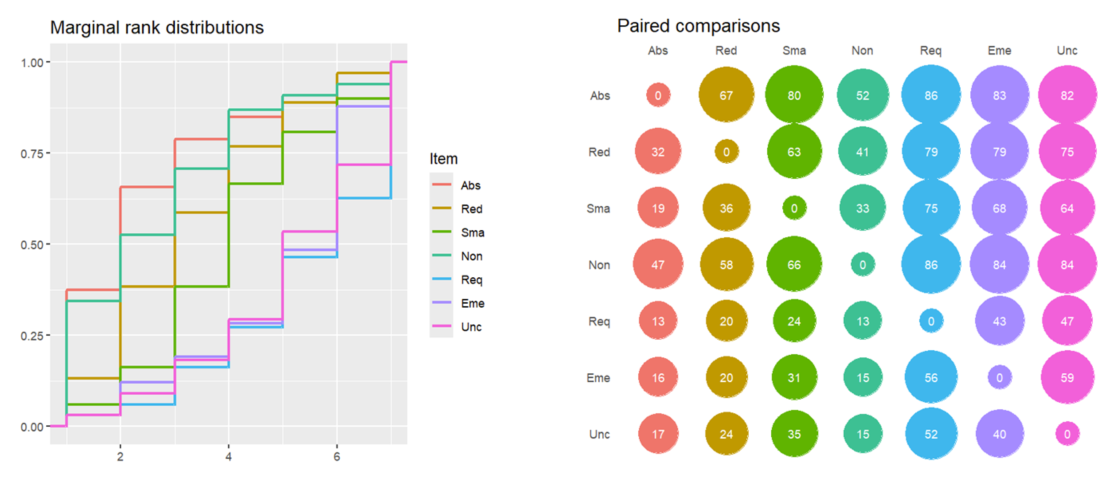
\includegraphics[width=\textwidth]{figures/RJ2025_paper_plotsanti.png}
          \caption{ECDFs of the marginal rank distributions (left) and bubble plot of the pairwise comparison matrix (right) for the Antifragility dataset. These plots correspond, respectively, to the elements named \code{ecdf} and \code{pc} of the output list returned by the generic method \code{plot.data\_descr}.}
        \label{fig:plot.data_descr}
\end{figure}


Concerning ranking data manipulation, \pkg{MSmix} provides functions designed to switch from complete to partial sequences, with the routine \code{data\_censoring}, or from partial to complete sequences, with the routines \code{data\_augmentation} and \code{data\_completion}. These functions are particularly useful in simulation scenarios for evaluating the robustness of inferential procedures in recovering the actual data-generating mechanisms under various types and extents of censoring and different data augmentation strategies for handling partial data.

With \code{data\_censoring}, complete rankings can be converted into partial rankings in two distinct ways. One approach obscures only the bottom ranks to produce a top partial ranking (set \code{topk = TRUE}), while the other obscures ranks at any position (set \code{topk = FALSE}). In both cases, users can specify how many positions are retained for each sequence through two schemes:
(i) a deterministic method, where an integer vector (of length $N$) is provided to the \code{nranked} argument specifying the desired number of ranks to be retained in each partial sequence; (ii) a stochastic method, where \code{nranked = NULL} (default) and a numeric vector is provided to the \code{probs} argument defining the $(n-1)$ probabilities associated with retaining different number of ranks (from 1 to $n-1$). These probabilities determine the random number of ranks to be retained in each partial sequence after censoring.\footnote{Recall that a partial sequence with $(n-1)$ observed entries corresponds to a full ranking.} An example of a deterministic top-$k$ censoring scheme is implemented below to covert the complete Antifragility ranking data into top-3 rankings.

\begin{example}
R> N <- nrow(ranks_AF)
R> top3_AF <- data_censoring(rankings = ranks_AF, topk = TRUE, nranked = rep(3,N))
R> top3_AF$part_rankings[1:3,]
  Abs Red Sma Non Req Eme Unc
1  NA   2   1   3  NA  NA  NA
2   1  NA   3   2  NA  NA  NA
3   3  NA   1   2  NA  NA  NA
> table(top3_AF$nranked)
 3
99
\end{example}
The output of \code{data\_censoring} is a list with a first component, named \code{part\_rankings}, corresponding to the input complete data matrix \code{rankings} with suitably censored (\code{NA}) entries, and a second component, named \code{nranked}, corresponding to the vector with the number of actually visible positions in each partial ranking.

An example of stochastic top-$k$ censoring scheme on the same dataset, that will result in a random number of bottom positions obscured, can be run as follows

\begin{example}
R> top_AF <- data_censoring(rankings = ranks_AF, topk = TRUE, probs = c(1:(n-2),0))
R> top_AF$part_rankings[1:3,]
  Abs Red Sma Non Req Eme Unc
1   4   2   1   3   5  NA  NA
2   1  NA   3   2  NA  NA  NA
3   3  NA   1   2  NA  NA  NA

R> table(top_AF$nranked)
 1  2  3  4  5
 1 14 16 19 49
\end{example}
In this case, the vector \code{probs} assigns an increasing chance of retaining a higher number of top positions, with the exception of a zero value in the last entry, forcing the non-occurrence of full rankings after censoring. Apart from the different setting for the \code{topk} argument, applying a censoring scheme to arbitrary positions requires a similar syntax to the top-$k$. The main difference is that, instead of the censoring process acting only on the bottom part of the rankings, the positions to be censored are determined uniformly at random once the number of ranks to be kept is specified by the user (either deterministically or stochastically).

We conclude this section with an illustration of the counterpart commands of \code{data\_censoring} available in \pkg{MSmix}, which act on partial rankings and fill in the missing positions with different criteria.
The first, called \code{data\_augmentation}, is the key function for estimating a MMS-mix on partial rankings via Algorithm \ref{alg:partial_mixture}. Here is a toy example with only two partial rankings characterized by different types of censoring.
\begin{example}
R> ranks_toy <- rbind(c(2, NA, 1, NA, 3), c(NA, 4, NA, 1, NA))
R> ranks_toy
     [,1] [,2] [,3] [,4] [,5]
[1,]    2   NA    1   NA    3
[2,]   NA    4   NA    1   NA

R> data_augmentation(rankings = ranks_toy)
[[1]]
     [,1] [,2] [,3] [,4] [,5]
[1,]    2    4    1    5    3
[2,]    2    5    1    4    3

[[2]]
     [,1] [,2] [,3] [,4] [,5]
[1,]    2    4    3    1    5
[2,]    3    4    2    1    5
[3,]    3    4    5    1    2
[4,]    2    4    5    1    3
[5,]    5    4    2    1    3
[6,]    5    4    3    1    2
\end{example}
The output list contains the matrices of all full rankings compatible with each partial sequence.\footnote{These correspond to the sets $\mathcal{C}(\bm r)$ introduced in Section 2.2.}
%\ref{ssec:partial}.}.
We remark that, despite the name \code{rankings} of the input (partially ranked) data matrix, the function \code{data\_augmentation} can also be applied to partial observations expressed in ordering format. In general, it supports the data augmentation of sequences containing at most 10 missing entries.

The second function, named \code{data\_completion}, completes each partial ranking with a single compatible full ranking. To complete the rankings in \code{ranks\_toy}, one needs to set the \code{ref\_rho} argument equal to a matrix of the same dimensions as \code{ranks\_toy}, containing the reference full rankings in each row. In the example below, we use the identity permutation and its opposite as the reference sequences for completion.
\begin{example}
R> data_completion(rankings = ranks_toy, ref_rho = rbind(1:5, 5:1))
     [,1] [,2] [,3] [,4] [,5]
[1,]    2    4    1    5    3
[2,]    5    4    3    1    2
\end{example}
The output is the matrix obtained by filling in the missing entries of each partial sequence with the relative positions of the unranked items according to the reference full ranking.\footnote{These sequences correspond to the result of data completion from the MC step described in Section
%\ref{ssec:partial}.}
2.2.}
The \code{data\_completion} command accommodates any type of censoring, similar to \code{data\_augmentation}, but without the need to enumerate all possible orders of missing positions. Consequently, there is no upper limit on the number of \code{NA} entries in the partial sequences.


%%%%
\subsection{Sampling}
\label{subsec:sampling}
The function devoted to simulating an i.i.d. sample of full rankings from a MMS-mix is \code{rMSmix}, which relies on the Metropolis-Hastings (MH) procedure implemented in the \textsf{R} package \pkg{BayesMallows} \citep{BayesMallows}. When $n\leq 10$, the routine also offers the possibility to perform exact sampling by setting the logical \code{mh} argument to \code{FALSE}.


The \code{rMSmix} function requires the user to specify: i) the desired number of rankings (\code{sample\_size}), ii) the number of items (\code{n\_items}) and iii) the number of mixture components (\code{n\_clust}). The mixture parameters can be separately passed with the (optional) arguments \code{rho}, \code{theta} and \code{weights}, set to \code{NULL} by default. If the user does not input the above parameters, the concentrations are sampled uniformly in the interval $(1/n^2,3/n^{3/2})$,\footnote{The concentration parameters play a delicate role. In fact, if $\theta$ is too close to zero, the MMS turns out to be indistinguishable from the uniform distribution on $\mathcal{P}_n$, while if $\theta$  is too large the MMS distribution would tend to a Dirac on the consensus ranking $\bm\rho$. The critical magnitude turns out to be $\theta\sim c/n^2$ with $c > 0$ fixed \citep{zhong2021mallows}.} while the simulation of the consensus parameters and the weights can be selected with the logical argument \code{uniform}. The option \code{uniform = TRUE} consists in generating the non-specified parameters uniformly in their support. Here is an example where $N=100$ full rankings of $n=8$ items are exactly generated from a 3-component MMS-mix, with assigned and equal concentrations $\bm\theta=(.15,.15,.15)$ and the other parameters sampled uniformly at random.
\begin{example}
R> sam_unif <- rMSmix(sample_size = 100, n_items = 8, n_clust = 3, theta = rep(.15, 3),
+               uniform = TRUE, mh = FALSE)
\end{example}

The function \code{rMSmix} returns a list of five named objects: the $N\times n$ matrix with the simulated complete rankings (\code{samples}), the model parameters actually used for the simulation (\code{rho}, \code{theta} and \code{weights}) and the simulated group membership labels (\code{classification}). For the previous example, they can be extracted as follows
\begin{example}
R> sam_unif$samples[1:3,]
     [,1] [,2] [,3] [,4] [,5] [,6] [,7] [,8]
[1,]    6    1    7    5    8    3    2    4
[2,]    2    1    3    7    5    4    8    6
[3,]    6    2    7    5    8    3    1    4

R> sam_unif$rho
     [,1] [,2] [,3] [,4] [,5] [,6] [,7] [,8]
[1,]    6    2    1    5    4    3    8    7
[2,]    4    2    5    3    8    7    1    6
[3,]    6    2    8    4    7    3    1    5

R> sam_unif$weights
[1] 0.49165535 0.04123627 0.46710838

R> table(sam_unif$classification)
 1  2  3
35  5 60
\end{example}
One can note that, with uniform sampling, cluster separation and balance of the drawings among the mixture components are not guaranteed. In fact, cluster 2 has a very small weight ($\omega_2 \approx 0.04$) corresponding to only 5 observations; moreover, the consensus rankings of clusters 2 and 3 are quite similar, as testified by their low relative Spearman distance obtained by dividing the output of command \code{spear\_dist} included in \pkg{MSmix} by the maximum value of the metric.\footnote{The maximum Spearman distance among two rankings of a given length $n$ is equal to $2\binom{n+1}{3}$.}
\begin{example}
R> max_spear_dist <- 2*choose(8+1,3)
R> spear_dist(rankings = sam_unif$rho[2,], rho = sam_unif$rho[3,])/max_spear_dist
[1] 0.1904762
\end{example}
To ensure separation among the mixture components and non-sparse weights, the user can set the option \code{uniform = FALSE}. Specifically, the consensus rankings are drawn with a minimum Spearman distance from each other equal to $\frac{2}{G}\binom{n+1}{3}$, and the mixing weights are sampled from a symmetric Dirichlet distribution with (large) shape parameters $\bm\alpha=(2G,\dots,2G)$ to favour populated and balanced clusters.
\begin{example}
R> sam_sep <- rMSmix(sample_size = 100, n_items = 8, n_clust = 3, theta = rep(.15, 3),
+               uniform = FALSE, mh = FALSE)
\end{example}
The three clusters are now more balanced and their central rankings have a larger relative distance.
\begin{example}
R> sam_sep$weights
[1] 0.5214495 0.2594782 0.2190723

R> spear_dist(rankings = sam_sep$rho)/max_spear_dist
     1         2
2 0.6309524
3 0.7023810 0.6666667
\end{example}
\begin{figure}[t]
     \centering
     \begin{subfigure}[b]{0.49\textwidth}
         \centering
         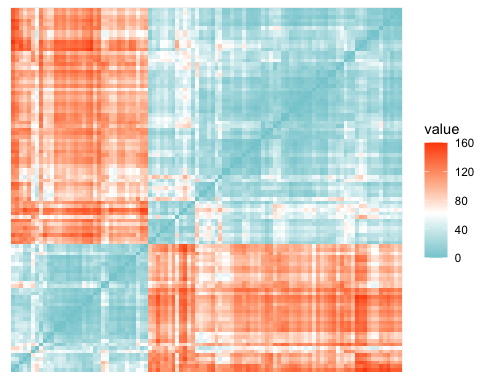
\includegraphics[width=\textwidth]{figures/RJ2025_paper_dist1_new.png}
         \caption{{Samples with uniformly generated parameters.}}
         \label{fig:s1a}
     \end{subfigure}
     \hfill
     \begin{subfigure}[b]{0.49\textwidth}
         \centering
         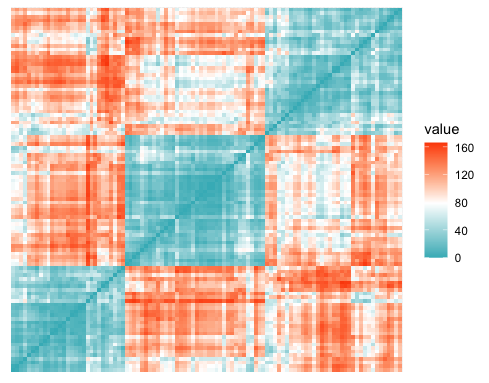
\includegraphics[width=\textwidth]{figures/RJ2025_paper_dist2_new.png}
         \caption{{Samples from separated clusters.}}
         \label{fig:s1b}
     \end{subfigure}
        \caption{{Heatmap of the Spearman distance matrix between all pairs of full rankings for two simulated samples from a 3-component MMS-mix, obtained by setting \code{uniform = TRUE} (a) and \code{uniform = FALSE} (b) in the \code{rMSmix} routine.}}
        \label{fig:s1}
\end{figure}
In Figure \ref{fig:s1}, we show the separation among clusters in the two examples through the Spearman distance matrix of the simulated samples, which quantifies the dissimilarity between each pair of observations. Specifically, Figures \ref{fig:s1a} and \ref{fig:s1b} can be constructed as follows\footnote{Notably, the \code{plot.dist} function of \pkg{MSmix} fills in the gap of a generic method for objects of class \code{"dist"} in \textsf{R}, since it allows to visualize, and hence compare, distance matrices of any metric.}
\begin{example}
R> plot(spear_dist(rankings = sam_unif$samples), show_labels = FALSE)
R> plot(spear_dist(rankings = sam_sep$samples), show_labels = FALSE)
\end{example}
{where the argument \code{show\_labels = FALSE} allows to drop the labels of the observations over the axes in the case of large samples.}
{The heatmaps indicate} the presence of only two well-separated clusters in the sample {obtained with uniformly generated parameters (Figure \ref{fig:s1a})}, while three groups are evident {when the simulation is performed by controlling the distance among components (Figure \ref{fig:s1b}).}

In conclusion, \code{rMSmix} is designed to facilitate the implementation of alternative sampling schemes, that can be fruitful to assess the performance of the inferential procedures and their robustness under a variety of simulation scenarios.


\subsection{Application on full rankings}
\label{subsec:est_full}
In this section, we show how to perform a mixture model analysis on the Antifragility rankings.
To this aim, we use the command \code{fitMSmix}, the core function of the \pkg{MSmix} package, which performs MLE of the MMS-mix on the input \code{rankings} via EM algorithm with the desired number \code{n\_clust} of components. The number of multiple starting points, needed to address the issue of local maxima, can be set through the argument \code{n\_start}, and the list \code{init} possibly allows to configure initial values of the parameters for each starting point.

The code below shows how to estimate the MMS-mix with a number of components ranging from 1 to 6 and save the values of the Bayesian information criterion (BIC) in a separate vector for then choosing the optimal number of clusters.
\begin{example}
R> FIT.try <- list()
R> BIC <- setNames(numeric(6), paste0('G = ', 1:6))
R> for(i in 1:6){
+    FIT.try[[i]] <- fitMSmix(rankings = ranks_AF, n_clust = i, n_start = 50)
+    BIC[i] <- FIT.try[[i]]$mod$bic}
\end{example}
The BIC values of the six estimated models are
\begin{example}
R> print(BIC)
   G = 1    G = 2    G = 3    G = 4    G = 5    G = 6
1494.435 1461.494 1442.749 1444.223 1449.714 1453.101
\end{example}
\begin{figure}[t]
\centering
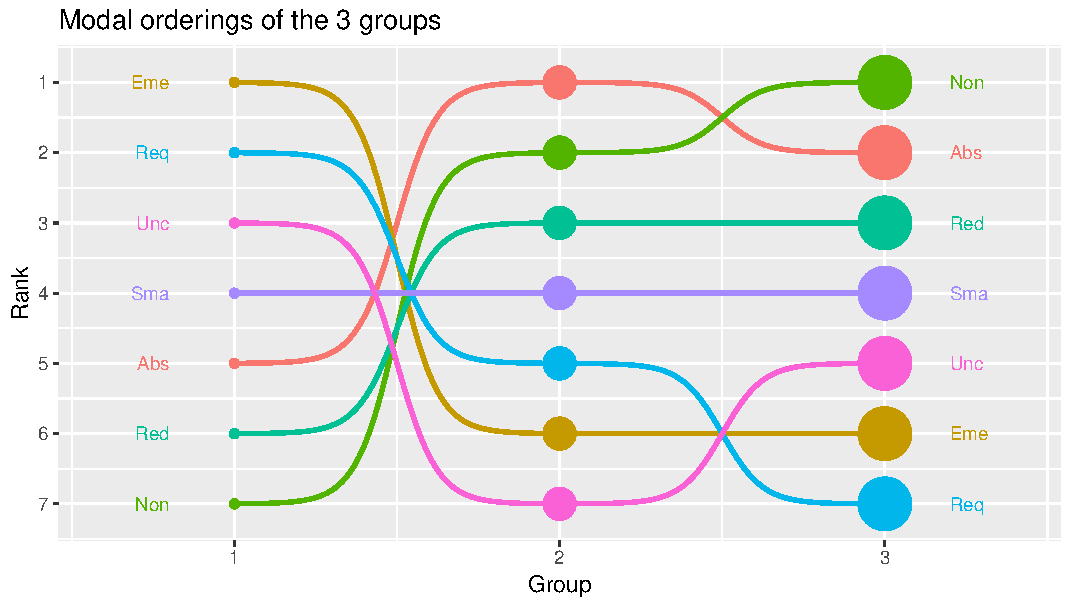
\includegraphics[width=0.8\textwidth]{figures/RJ2025_paper_cons.pdf}
\caption{Bump plot depicting the estimated consensus rankings of the ${G}=3$ clusters for the \code{ranks\_antifragility} dataset. This plot corresponds to the element named \code{bump\_plot} of the output list returned by the generic method \code{plot.emMSmix}.}
 \label{f:antifr_plot1}
\end{figure}
suggesting \code{G = 3} as the optimal number of groups (lowest BIC).
The function \code{fitMSmix} creates an object of S3 class \code{"emMSmix"}, which is a list whose main component, named  \code{mod}, describes the best fitted model over the \code{n\_start} initializations. It includes, for example, the MLE of the parameters (\code{rho}, \code{theta} and \code{weights}), the fitting measures (\code{log\_lik} and \code{bic}), the estimated posterior membership probabilities (\code{z\_hat}) and the related MAP allocation (\code{map\_classification}) as well as the binary indicator of convergence achievement (\code{conv}).

The MLEs of the best fitted model can be shown also through the generic method \code{summary.emMSmix},
\begin{example}
R> summary(object = FIT.try[[3]])
Call:
fitMSmix(rankings = ranks_AF, n_clust = 3, n_start = 50)

-----------------------------
--- MLE of the parameters ---
-----------------------------

Component-specific consensus rankings:
       Abs Red Sma Non Req Eme Unc
Group1   5   6   4   7   2   1   3
Group2   1   3   4   2   5   6   7
Group3   2   3   4   1   7   6   5

Component-specific consensus orderings:
       Rank1 Rank2 Rank3 Rank4 Rank5 Rank6 Rank7
Group1 "Eme" "Req" "Unc" "Sma" "Abs" "Red" "Non"
Group2 "Abs" "Non" "Red" "Sma" "Req" "Eme" "Unc"
Group3 "Non" "Abs" "Red" "Sma" "Unc" "Eme" "Req"

Component-specific precisions:
Group1 Group2 Group3
 0.111  0.241  0.087

Mixture weights:
Group1 Group2 Group3
 0.083  0.343  0.574
\end{example}
which also displays the estimated modal orderings in the rows of the second output matrix. The generic function \code{plot.emMSmix} is also associated to the class \code{"emMSmix"} and constructs a list of two fancy plots, see commands below.
\begin{example}
R> p_fit3_AF <- plot(FIT.try[[3]])
R> p_fit3_AF$bump_plot()
R> p_fit3_AF$est_clust_prob()
\end{example}
The first one is the bump plot (Figure \ref{f:antifr_plot1}) depicting the consensus ranking of each cluster, with different colors assigned to each item, circle sizes proportional to the estimated weights and lines to better highlight item positions in the modal orderings of the various components. For this example, we note that the size of the second cluster is almost half that of the third cluster, while the first cluster is very small. Moreover, the two larger groups (2 and 3) exhibit very similar modal rankings and quite opposite preferences with respect to the first cluster (items such as ``Emergence'', ``Requisite variety'', and ``Uncoupling'' are ranked at the top in cluster 1, but placed at the bottom in groups 2 and 3).

Figure \ref{f:antifr_plot2} shows, instead, the individual cluster memberships probabilities, describing the uncertainty with which each observation could be assigned to the mixture components. For example, the units 10, 15, 19, 20, 71, 74, 78 and 94 have high probabilities (close to 1) of belonging to group 1. Instead, some units (e.g., unit 8, 28, 36, and 44) have similar membership probabilities of belonging to clusters 2 or 3, indicating less confidence in their assignment to one of the two groups. On the other hand, when some clusters are close on the ranking space, a certain degree of uncertainty in recovering the true membership is expected.

\begin{figure}[t]
\centering
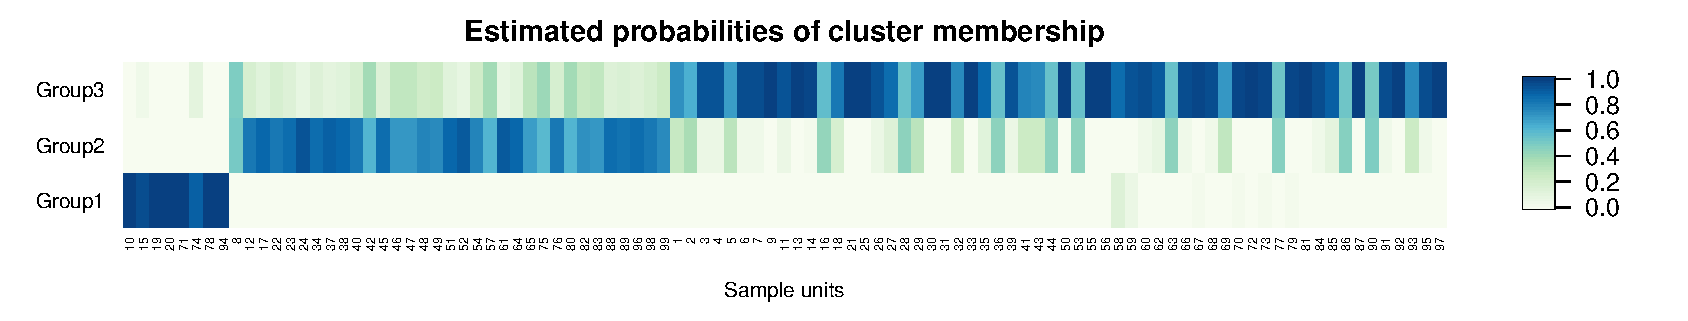
\includegraphics[width=\textwidth]{figures/RJ2025_paper_zeta.pdf}
\caption{Heatplot of the estimated cluster membership probabilities for each observation of the \code{ranks\_antifragility} dataset. This plot corresponds to the element named \code{est\_clust\_prob} of the output list returned by the generic method \code{plot.emMSmix}.}
 \label{f:antifr_plot2}
\end{figure}
The package provides also routines for computing the CIs, working with the object of class \code{"emMSmix"} as first input argument. For example, we can produce asymptotic CIs for the precisions and mixture weights with \code{confintMSmix}, which is a function specific for full ranking data. With the default confidence level (\code{conf\_level = 0.95}), one obtains
\begin{example}
R> confintMSmix(object = FIT.try[[3]])
Asymptotic 95%CIs for the precisions:
       lower upper
Group1 0.000 0.226
Group2 0.153 0.329
Group3 0.068 0.106

Asymptotic 95%CIs for the mixture weights:
       lower upper
Group1 0.021 0.144
Group2 0.195 0.491
Group3 0.473 0.676
\end{example}

Another possibility relies on bootstrap CI calculation. Let us opt for the soft bootstrap method (the default choice when $G>1$) which, unlike the separated one (\code{type = "separated"}), produces CIs also for weights. We require \code{n\_boot = 500} bootstrap samples and then print the output object of class \code{"bootMSmix"} through the generic function \code{print.bootMSmix}.
\begin{example}
R> CI_bootSoft <- bootstrapMSmix(object = FIT.try[[3]], n_boot = 500, all = TRUE)
R> print(CI_bootSoft)
Bootstrap itemwise 95%CIs for the consensus rankings:

       Abs           Red         Sma           Non     Req         Eme
Group1 "{3,4,5,6,7}" "{4,5,6,7}" "{2,3,4,5,6}" "{6,7}" "{1,2,3,4}" "{1,2}"
Group2 "{1}"         "{2,3}"     "{4}"         "{2,3}" "{5}"       "{6}"
Group3 "{1,2,3}"     "{2,3}"     "{4,5}"       "{1,2}" "{7}"       "{5,6}"
       Unc
Group1 "{2,3,4,5}"
Group2 "{7}"
Group3 "{4,5,6}"

Bootstrap 95%CIs for the precisions:
       lower upper
Group1 0.068 0.212
Group2 0.193 0.314
Group3 0.069 0.112

Bootstrap 95%CIs for the mixture weights:
       lower upper
Group1 0.071 0.101
Group2 0.283 0.404
Group3 0.505 0.636
\end{example}
The logical argument \code{all} indicates whether the MLEs estimates obtained from the  bootstrap samples must be returned in the output. When \code{all = TRUE}, as in this case, the user can visualize the bootstrap sample variability with the generic function \code{plot.bootMSmix}. It returns a list with the heatmap of the first-order marginals of the bootstrap samples, and the kernel densities for the precisions and weights. For this application, the latter two plots (Figure~\ref{fig:boot_theta_weights}) are obtained as follows.
\begin{example}
R> p_ci_soft <- plot(CI_bootSoft)
R> p_ci_soft$theta_density()
R> p_ci_soft$weights_density()
\end{example}


\begin{figure}[t]
     \centering
     \begin{subfigure}[b]{0.49\textwidth}
         \centering
         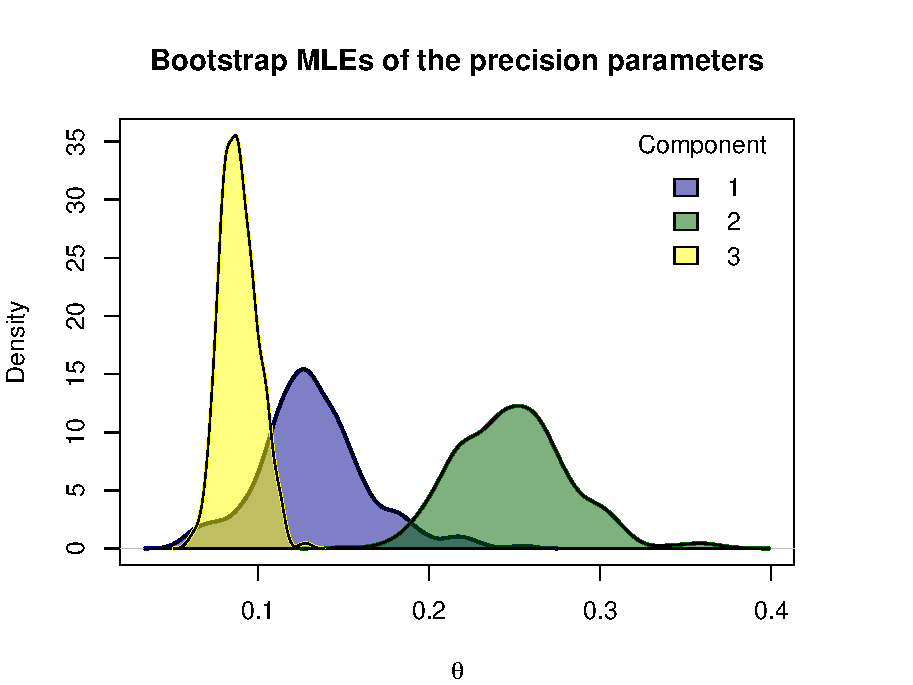
\includegraphics[width=\textwidth]{figures/RJ2025_paper_boot1.pdf}
     \end{subfigure}
 %    \hfill
     \begin{subfigure}[b]{0.49\textwidth}
         \centering
         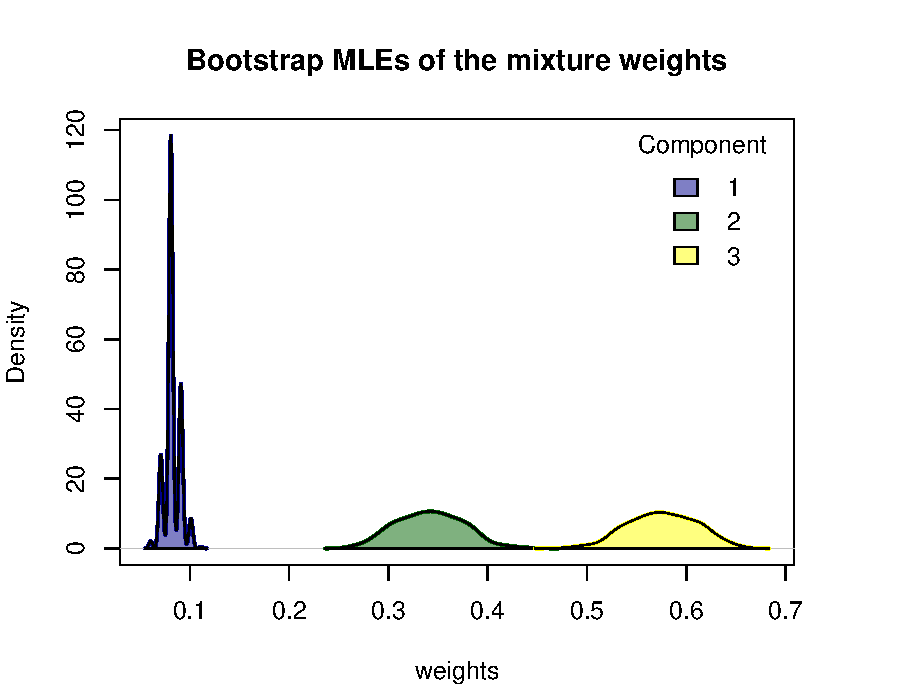
\includegraphics[width=\textwidth]{figures/RJ2025_paper_boot2.pdf}
      \end{subfigure}

        \caption{Kernel densities of the soft bootstrap MLEs of the precision parameters (left) and the weights (right) for the \code{ranks\_antifragility} dataset. These plots correspond, respectively, to the elements named \code{theta\_density} and \code{weights\_density} of the output list returned by the generic method \code{plot.bootMSmix}.}
        \label{fig:boot_theta_weights}
\end{figure}



\subsection{Application on partial rankings}
\label{subsec:est_partial}

In this section, we illustrate how to perform inference on the partial rankings collected in the original \code{ranks\_beers} dataset.
These data were gathered through an online survey administered to the participants of the 2018 Pint of Science festival held in Grenoble. A sample of $N = 105$ subjects provided their partial rankings of $n=20$ beers according to their personal tastes. The partial rankings, characterized by different censoring patterns (that is, not exclusively top-$k$ sequences), are recorded in the first 20 columns of the dataset, while column 21 contains a covariate regarding respondents' residency.

The barplot with the percentages of the number of beers actually ranked by the participants is reported in Figure \ref{fig:descr_beers}. We restrict the analysis to partial rankings with maximum 8 missing positions, to show both the data augmentation schemes (Algorithms \ref{alg:partial_mixture} and \ref{alg:partial_mcem}) implemented in the package. {Note that, since our EM algorithms rely on the MAR assumption, we preliminarily conducted an empirical evaluation to assess whether the realized missingness pattern significantly deviates from this hypothesis. This check is described in Appendix A3.}

Thanks to the \code{subset} argument of \code{fitMSmix}, we can specify the subsample of observations to be considered directly in the fit command.
To speed up the estimation process, we parallelize the multiple starting points by setting  \code{parallel = TRUE}.\footnote{Note that exact reproducibility of this section may not be possible due to the use of parallelization, which can lead to minor variations in inferential results between runs.}

\begin{example}
R> rankings <- ranks_beers[,1:20]
R> subset_beers <- (rowSums(is.na(rankings)) <= 8)
R> library(doParallel)
R> registerDoParallel(cores = detectCores())
R> FIT_aug <- fitMSmix(rankings,n_clust = 1, n_start = 15,
+                     subset = subset_beers, mc_em = FALSE, parallel = TRUE)
R> FIT_mcem <- fitMSmix(rankings, n_clust = 1, n_start = 15,
+                      subset = subset_beers, mc_em = TRUE, parallel = TRUE)
\end{example}
%
\begin{figure}[t]
     \centering
     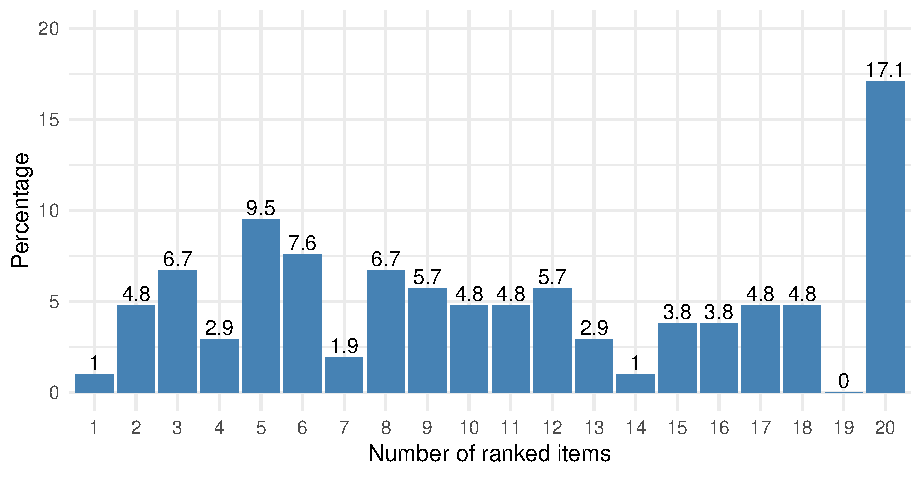
\includegraphics[width=0.65\textwidth]{figures/RJ2025_paper_descr_beers.pdf}
      \caption{Percentages of the number of ranked items in the \code{ranks\_beers} dataset. This barplot corresponds to the element named \code{n\_ranked\_distr} of the output list returned by the generic method \code{plot.data\_descr}.}
     \label{fig:descr_beers}
\end{figure}
The logical \code{mc\_em} argument indicates whether the MCEM scheme (Algorithm \ref{alg:partial_mcem}) must be applied. When \code{mc\_em = FALSE} (default),  Algorithm \ref{alg:partial_mixture} is implemented.\footnote{
This type of data augmentation is supported for up to 10 missing positions in the partial rankings. However, it is important to note that while this operation may be feasible in principle for some datasets, it can be slow and memory-intensive. For instance, augmenting and storing all rankings compatible with the subset of the beers dataset with a maximum of 10 missing positions requires more than 3GB of storage space.}
We note that, for this application, the results of the two methods are very similar.

\begin{example}
R> spear_dist(FIT_aug$mod$rho,FIT_mcem$mod$rho)/(2*choose(20+1,3))
[1] 0.001503759

R> c('theta_aug' = FIT_aug$mod$theta, 'theta_mcem' = FIT_mcem$mod$theta)
  theta_aug  theta_mcem
0.008580397 0.008964391
\end{example}

One can then evaluate the uncertainty associated to the consensus ranking estimated via the MCEM with the non-parametric bootstrap (default for $G=1$). Also in this case, we can parallelize over the multiple starting points of the EM algorithm used to fit the bootstrap samples.
\begin{example}
R> boot_mcem <- bootstrapMSmix(object = FIT_mcem, n_boot = 300, n_start = 15,
                             all = TRUE, parallel = TRUE)

R> print(boot_mcem)
Bootstrap itemwise 95%CIs for the consensus rankings:

       Stella                   Kwak          KronKron  Faro
Group1 "{12,13,14,15,16,17,18}" "{2,3,4,5,6}" "{19,20}" "{8,9,10,11,12,13,14,15}"
       Kron1664           Chimay  Pelforth           KronCarls
Group1 "{14,15,16,17,18}" "{1,2}" "{11,12,13,14,15}" "{12,13,14,15,16,17,18}"
       KronKanter Hoegaarden           Grimbergen      Pietra
Group1 "{19,20}"  "{6,7,8,9,10,11,12}" "{2,3,4,5,6,7}" "{6,7,8,9,10,11,12,13}"
       Affligem         Goudale           Leffe             Heineken
Group1 "{3,4,5,6,7,8}" "{4,5,6,7,8,9,10}" "{6,7,8,9,10,11}" "{14,15,16,17,18}"
       Duvel             Choulette                Orval
Group1 "{2,3,4,5,6,7,8}" "{12,13,14,15,16,17,18}" "{5,6,7,8,9,10,11,12,13,15}"
       Karmeliet
Group1 "{1,2,3,4,5,6}"

Bootstrap 95%CIs for the precisions:
       lower upper
Group1 0.007 0.013
R> plot(boot_mcem)$rho_heatmap()
\end{example}
The heatmap of the bootstrap output, displayed in Figure \ref{fig:heat_beers}, helps in understanding the variability and confidence in the rankings of the beers. In fact, the top ranked beer (Chimay) and the two bottom ranked ones (KronKanter and KronKron) are quite reliably ranked in those positions. On the contrary, the ranks of the other beers are more uncertain, with itemwise  95\% bootstrap-based CIs for some beers being as wide as 10 positions (out of 20). Note also that some itemwise regions can result in subsets of non-contiguous ranks, as in the case of \code{Orval} whose CI does not include rank 14.
%
\begin{figure}[t]
     \centering
     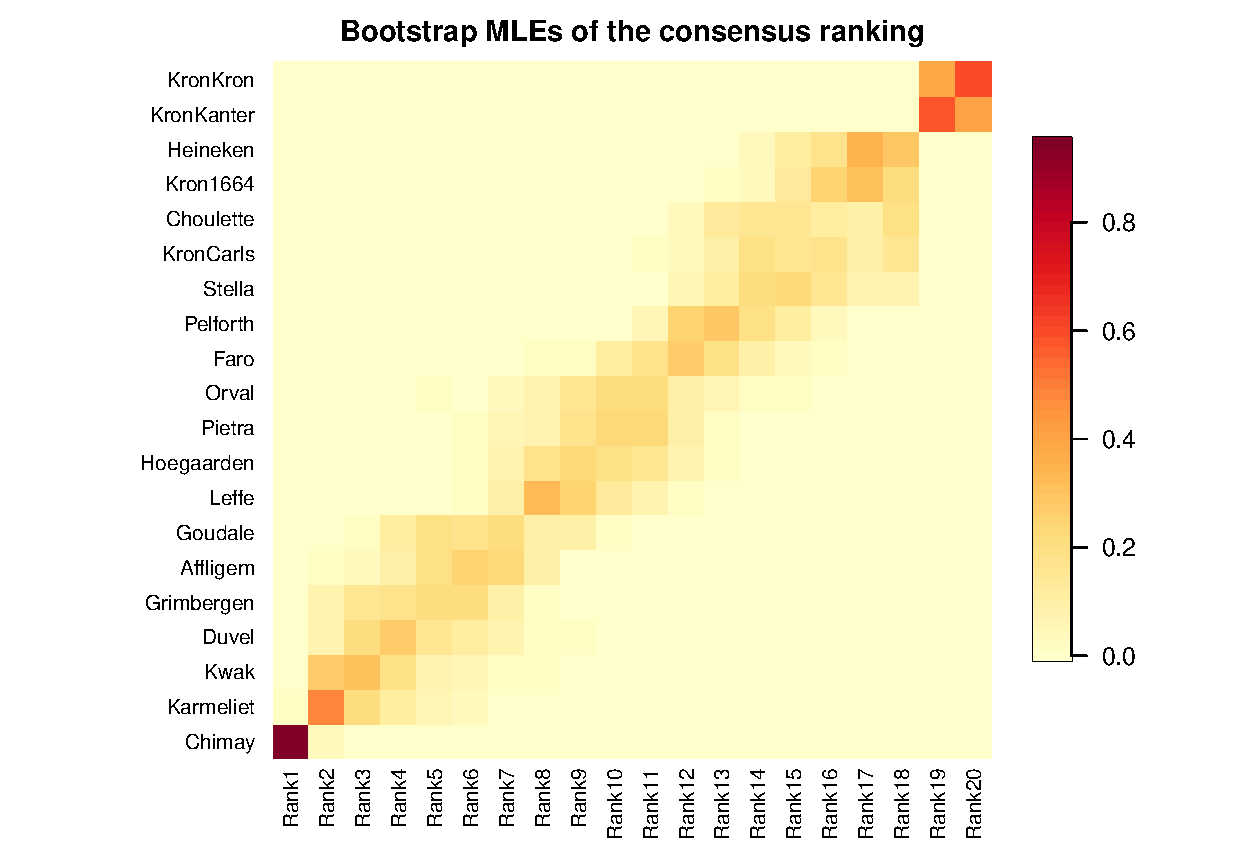
\includegraphics[scale=0.7,width=0.9\textwidth]{figures/RJ2025_paper_heat.pdf}
      \caption{Heatmap of the bootstrap MLE of the consensus ranking for a subsample of the \code{ranks\_beers} dataset. On the y-axis, items are ordered according to the MLE of $\bm\rho$ (top-ranked beer at the bottom). This plot corresponds to the element named \code{rho\_heatmap} of the output list returned by the generic method \code{plot.bootMSmix}.}
     \label{fig:heat_beers}
\end{figure}
%
We conclude this section by stressing that the application to the beers dataset represents a non-trivial case of ranking data analysis, since currently there are no other \textsf{R} packages supporting MLE of the MM on partially-ranked sequences with arbitrary missing positions.



\subsection{Additional options}

The \pkg{MSmix} package also supplies some functions to deal with the distribution of the Spearman distance. Although these functions are primarily used internally to fit the model (see the algorithms in Appendix A1), they are made available for external use due to their standalone utility.


The function \code{spear\_dist\_distr} returns the (log-)frequency distribution of the Spearman distance under the uniform model. If $n\leq 20$, the function returns the exact distribution by relying on a call to the \code{get\_cardinalities} routine of \pkg{BayesMallows}. Here is an example with $n=5$.
\begin{example}
R> spear_dist_distr(n_items = 5)
$distances
 [1]  0  2  4  6  8 10 12 14 16 18 20 22 24 26 28 30 32 34 36 38 40
$logcard
 [1] 0.000000 1.386294 1.098612 1.791759 1.945910 1.791759 1.386294 2.302585
 [9] 1.791759 2.302585 1.791759 2.302585 1.791759 2.302585 1.386294 1.791759
[17] 1.945910 1.791759 1.098612 1.386294 0.000000
\end{example}
When $n> 20$, the approximate distribution introduced by \cite{crispino23efficient} is returned and, in the case $n\geq 170$, its calculation is restricted over a fixed grid of values of the Spearman distance to limit computational burden.

The functions \code{partition\_fun\_spear},  \code{expected\_spear\_dist} and \code{var\_spear\_dist} provide, respectively, the partition function $Z(\theta)$, the expected value $\mathbb{E}_{\theta}[D]$ and the variance $\mathbb{V}_{\theta}[D]$ of the Spearman distance under the MMS. For $n=5$, one has
\begin{example}
R> partition_fun_spear(theta = 0.1, n_items = 5)
[1] 3.253889
R> expected_spear_dist(theta = 0.1, n_items = 5)
[1] 2.421115
R> var_spear_dist(theta = 0.1, n_items = 5)
[1] 4.202741
\end{example}
For these functions, the computation is exact or approximate according to the same principle described for \code{spear\_dist\_distr}.


\section{Conclusions}
\label{sec:concl}
The new \pkg{MSmix} package enriches the \textsf{R} software environment with functions to analyze finite mixtures of MMS on full and partial rankings with arbitrary patterns of censoring. Inference is conducted within the ML framework via EM algorithms. Estimation uncertainty is quantified with bootstrap methods and approximate CIs from the asymptotic likelihood theory.

The innovative contributions of \pkg{MSmix} span from both methodological and computational advancements to address the lacks and limitations found in most of the existing packages, especially the possibility of realizing a ranking data analysis with many items and missing positions or assessing estimation uncertainty of model parameters. Moreover, the estimation procedures have been generalized and optimized to work effectively across a spectrum of censoring patterns, rather than being limited solely to the top-$k$ scenario.
The package also exploits the construction of S3 class objects and related generic methods to offer a unified and original analysis framework. In this regard, a special attention was devoted to the development of effective visualization tools and summaries, that can assist the users in the reporting results and designing conclusions with a more transparent account of the associated uncertainty.

Our inferential procedures rely on EM algorithms assuming a MAR missing data mechanism. Under the MAR assumption, missingness does not depend on the unobserved preferences, allowing the EM algorithm to yield unbiased estimates without explicitly modeling the missing data process \citep{rubin1976inference,little2019statistical}. Although MAR is a common simplifying assumption in partial ranking analysis \citep{beckett93maximum,Jacques2014,piancastelli2025time}, it may not hold in real-world settings. For instance, top-$k$ rankings can arise when respondents omit to rank certain items due to unfamiliarity or low popularity, indicating that missingness depends on unobserved preferences and could, thus, significantly depart from the pure MAR assumption. It is well known that ignoring the missingness process under non-MAR scenarios can bias estimates obtained from standard EM algorithms \citep{little2019statistical}. However, the effects of MAR violations on the estimation accuracy of EM algorithms, as well as methods to address non-ignorable missingness, remain largely unexplored in the partial ranking literature. In this context, extending the methods provided by \pkg{MSmix} to better handle missing data in ranking models would represent a valuable methodological contribution for future research.

The package architecture and its computational achievements can facilitate code extensibility for accomplishing these innovative directions. For example, its flexibility in accommodating diverse data censoring patterns could be of support for exploring the plausibility of the standard MAR assumption or developing extensions of parametric mixture models incorporating non-ignorable missing data mechanisms. Moreover, the package capability to analyze data characterized by a large number of alternatives could motivate the interest in clustering similar items, as recently proposed for the MM in \citet{piancastelli}, or even in developing methods to solve bi-clustering problems.  Finally, to better characterize choice processes, the EM algorithms could be integrated with an additional step for estimating the impact of individual and/or item-specific covariates - a typical but complex task in preference analysis from ranking data \citep[see e.g.,][]{ gormley2008mixture,zhu21partition}.
We are currently working in this direction with a proposal to enrich the MMS-mix with a \textit{Mixture of Experts} model \citep{jacobs,jordan}, that is, a mixture model in which the weights are functions of the covariates \citep{crispinoMoE}. Future releases of \pkg{MSmix} will also include functions to deal with different distances among rankings.

\section{Acknowledgments}
The authors would like to thank the anonymous
reviewers for their constructive and insightful comments that greatly
improved the manuscript and the package. The authors wish to thank Prof. Luca Tardella and Prof. Enrico Casadio Tarabusi for the insightful discussions on various aspects of the methodology used in this paper. Additionally, the authors wish to thank Prof Maria Vincenza Ciasullo, Dr. Nicola Cucari, Dr. Raffaella Montera, Prof Maria Iannario and Prof. Rosaria Simone for generously sharing their data. \\ The opinions expressed are those of the authors and do not necessarily reflect the views of the Bank of Italy or the Eurosystem.

\bibliography{RJ2025_paper}

\address{Marta Crispino\\
  Department of Economics, Statistics and Research\\
  Bank of Italy, Rome, Italy\\
  \email{marta.crispino@bancaditalia.it}
  }

\address{Cristina Mollica\\
 Department of Statistical Sciences\\
 Sapienza University of Rome, Italy\\
  \email{cristina.mollica@uniroma1.it}
  }

\address{Lucia  Modugno\\
 Department of Economics, Statistics and Research\\
  Bank of Italy, Rome, Italy\\
  \email{lucia.modugno@bancaditalia.it}
  }

\newpage
\renewenvironment{example}{\itshape \small \begin{quote}}{\end{quote}}

\section{Appendix}
\label{sec:appendix}

\subsection{Estimation algorithms}
\label{app:Algo}
We here provide the pseudo-code of the estimation algorithms implemented in \pkg{MSmix}. In the heterogeneous case ($G>1$), the latent group membership of the $l$-th distinct observed ranking $\bm{r}_l$ is denoted with $\bm z_l = (z_{l1},\dots, z_{lG})$, where $z_{lg} = 1$ if the observation belongs to component $g$ and $z_{lg} = 0$ otherwise.

\begin{algorithm}[h]\small
\caption{MLE of the MMS parameters from full rankings}
\label{alg:full}
\hspace*{\algorithmicindent} \textbf{Input}: $\underline{\bm{r}}=\{\bm{r}_1,\dots,\bm{r}_N\}$ full $n$-rankings.
\begin{enumerate}
    \item[] \textbf{Preliminary steps}:
\begin{itemize}
    \item[-] For $l=1,\dots,L$, compute the frequency $N_l$ of each distinct observed ranking $\bm{r}_l$.
    \item[-] Compute either the exact or the
approximate frequency distribution of the Spearman distance $\{d,N_d\}_{d\in\mathcal{D}_n}$.
    \end{itemize}
    \item Compute the MLE of the consensus ranking $\bm\rho$:
    \begin{enumerate}
        \item Compute the sample mean rank vector ${\bm{\bar r}}=(\bar{r}_1,\ldots,\bar{r}_n)$.
        \item Compute $\hat{\bm{\rho}}=\text{rank}({\bm{\bar r}})$.
    \end{enumerate}
    \item Compute the MLE of the concentration parameter $\theta$:
    \begin{enumerate}
        \item  Compute the sample average distance $\bar d=\frac{1}{N}\sum_{l=1}^LN_ld(\bm{r}_l,\hat{\bm{\rho}})=2(c_n-\hat{\bm{\rho}}^T{\bm{\bar r}})$.
        \item  Apply \code{uniroot} to find the solution of the equation $\mathbb{E}_{\theta}(D) = 2(c_n-\hat{\bm{\rho}}^T{\bm{\bar r}})$ in $\theta$.
    \end{enumerate}
\end{enumerate}
    \hspace*{\algorithmicindent} \textbf{Output}: $\hat{\bm{\rho}}$ and $\hat{\theta}$.
\end{algorithm}


\begin{algorithm}[h]\small
\caption{MLE of the MMS-mix parameters from full rankings}
\label{alg:full_mixture}
\hspace*{\algorithmicindent} \textbf{Input}: $\underline{\bm{r}}=\{\bm{r}_1,\dots,\bm{r}_N\}$ full $n$-rankings; $G$ number of clusters; $\underline{\bm{\rho}}^{(0)}, \bm{\theta}^{(0)}, \bm{\omega}^{(0)}$ initial values.

\begin{enumerate}
\item[] \textbf{Preliminary steps}:
\begin{itemize}
    \item[-] For $l=1,\dots,L$, compute the frequency $N_l$ of each distinct observed ranking $\bm{r}_l$.
    \item[-] Compute either the exact or the
approximate frequency distribution of the Spearman distance $\{d,N_d\}_{d\in\mathcal{D}_n}$.
    \end{itemize}

     \item[] Repeat the E- and M-step below until convergence:
    \item[] \textbf{E-step}: for $l=1,\dots,L$ and $g=1,\dots,G$, compute
$ \hat z_{lg} = \frac{\hat\omega_g\mathbb{P}(\bm{r}_l\,|\hat{\bm{\rho}}_g,\hat\theta_g)}{\sum_{g\prime=1}^G\hat\omega_{g\prime}\mathbb{P}(\bm{r}_l\,|\hat{\bm{\rho}}_{g\prime},\hat\theta_{g\prime})}$.
    \item[]\textbf{M-step}: for $g=1,\dots,G$ compute
    \begin{enumerate}
        \item $\hat \omega_g =\hat{N}_g/N$ with $\hat{N}_g =\sum_{l=1}^L N_l \hat z_{lg}$.
        \item The MLE of $\bm\rho_g$ as in step 1 of Algorithm \ref{alg:full},  by replacing $\bar{\bm r}$ with\\
        $\bar{\bm r}_g = (\bar r_{g1},\dots, \bar r_{gn})$, where $\bar r_{gi} = \frac{1}{\hat N_g}\sum_{l=1}^L N_l\hat z_{lg}r_{li}$.
        %{\color{blue}Marta: in realtà qui secondo me non facciamo così ma usiamo hard clustering --> check}
        \item The MLE of $\theta_g$ as in step 2 of Algorithm \ref{alg:full}, by replacing $\bar{\bm r}$ with $\bar{\bm r}_g$ and $\hat{\bm\rho}$ with $\hat{\bm\rho}_g$.
    \end{enumerate}
\end{enumerate}
    \hspace*{\algorithmicindent} \textbf{Output}: $\underline{\hat{\bm{\rho}}}=\{\hat{\bm{\rho}}_1,\dots,\hat{\bm{\rho}}_G\},{\hat{\bm\theta}}=\{\hat{\theta}_1,\dots,\hat{\theta}_G\},{\hat{\bm\omega}}=\{\hat\omega_1,\dots,\hat\omega_G\}$, and $\underline{\hat{\bm z}}=\{\bm \hat z_1,\dots,\bm \hat z_N\}$.
\end{algorithm}



\begin{algorithm}[h!]\small
\caption{MLE of the MMS-mix parameters from partial rankings}
\label{alg:partial_mixture}
\hspace*{\algorithmicindent} \textbf{Input}: $\underline{\bm{r}}=\{\bm{r}_1,\dots,\bm{r}_N\}$ partial $n$-rankings; $G$ number of clusters; $\underline{\bm{\rho}}^{(0)}, \bm{\theta}^{(0)}, \bm{\omega}^{(0)}$ initial values.
\begin{enumerate}
\item[] \textbf{Preliminary steps}: for $l=1,\dots,L$,
\begin{itemize}
    \item[-] compute the frequency $N_l$ of each distinct observed ranking $\bm{r}_l$.
    \item[-] Compute and store the sets $\mathcal{C}(\bm r_l)$ of full rankings compatible with each distinct $\bm{r}_l$.
\end{itemize}
     \item[] Repeat the E- and M-step below until convergence:
    \item[] \textbf{E-step}:
    \begin{enumerate}
        \item For each distinct $\bm r_l$ with $l=1,\dots,L$ and for each $\bm{r}^*_{m^\prime}\in\mathcal{C}(\bm r_l)$, compute
        \vspace{-1mm}
$$\hat{p}_{lm^\prime}=\mathbb{P}(\bm{r}^*_{m^\prime}\,|\bm{r}_l,\underline{\hat{\bm{\rho}}},{\hat{\bm\theta}},{\hat{\bm\omega}})
=\frac{\sum_{g=1}^G \hat\omega_g e^{-2\hat\theta_g\left(c_n-{\hat{\bm{\rho}}_g^T}\bm{r}^*_{m^\prime}\right)-\log Z\left(\hat\theta_g\right)}}{\sum_{\bm{s}^*\in \mathcal{C}(\bm{r}_l)}\sum_{g=1}^G \hat\omega_ge^{-2\hat\theta_g\left(c_n-\hat{\bm{\rho}}^T_{g}\bm{s}^*\right)-\log Z\left(\hat\theta_g\right)}}
.$$
\vspace{-3mm}
\item For $m=1,\dots,M$, compute
$
\hat{N}_m=\sum_{l:\,\bm{r}^*_{m^\prime}\in\mathcal{C}(\bm{r}_l)} N_l \hat{p}_{lm^\prime}
$.
\vspace{-3mm}
        \item For $m=1,\dots,M$, and $g=1,\dots,G$, compute
$\hat z_{mg}=\dfrac{\hat\omega_g\mathbb{P}\big(\bm{r}^*_m\big\vert\hat{\bm{\rho}}_g,\hat\theta_g\big)}{\sum_{g'=1}^G\hat\omega_{g'}\mathbb{P}\big(\bm{r}^*_m\big\vert\hat{\bm{\rho}}_{g'},\hat\theta_{g'}\big)}$.
\vspace{-3mm}
    \end{enumerate}
    \item[] \textbf{M-step}: for $g=1,\dots,G$, compute
    \begin{itemize}
        \item[-] $\hat\omega_g =\hat{N}_g/N$ with $\hat{N}_g=\sum_{m=1}^M\hat{N}_m\hat z_{mg}$.
        \item[-] The MLE of $\bm\rho_g$ as in M-step (b) of Algorithm \ref{alg:full_mixture},  by replacing $\bar{\bm r}_g$ with\\
        $\bar{\bm r}^*_g = (\bar r^*_{g1},\dots, \bar r^*_{gn})$, where $\bar r^*_{gi} = \frac{1}{\hat N_g}\sum_{m=1}^M \hat N_m \hat z_{mg}r^*_{mi}$.
        \item[-] The MLE of $\theta_g$ as in M-step (c) of Algorithm \ref{alg:full_mixture}, by substituting $\bar{\bm r}_g$ with $\bar{\bm r}^*_g$.
    \end{itemize}
\end{enumerate}
   \hspace*{\algorithmicindent} \textbf{Output}: $\underline{\hat{\bm{\rho}}}=\{\hat{\bm{\rho}}_1,\dots,\hat{\bm{\rho}}_G\},{\hat{\bm\theta}}=\{\hat{\theta}_1,\dots,\hat{\theta}_G\},{\hat{\bm\omega}}=\{\hat\omega_1,\dots,\hat\omega_G\}\text{ and }\underline{\hat{\bm z}}=\{\bm \hat z_1,\dots,\bm \hat z_N\}$.
\end{algorithm}


\begin{algorithm}[h!]\small
\caption{MLE of the MMS-mix parameters from partial rankings (MCEM)}
\label{alg:partial_mcem}
\hspace*{\algorithmicindent} \textbf{Input}: $\underline{\bm{r}}=\{\bm{r}_1,\dots,\bm{r}_N\}$ partial $n$-rankings; $G$ number of clusters; $\underline{\bm{\rho}}^{(0)}, \bm{\theta}^{(0)}, \bm{\omega}^{(0)}$ initial values.


\begin{enumerate}
\item[] \textbf{Preliminary step}: for $s=1,\dots,N$, complete $\bm{r}_s$ at random, obtaining a full ranking $\bm{r}^*_s\in \mathcal{C}(\bm r_s)$.
    \item[] Repeat the E-, M- and MC-step below until convergence:
    \item[] \textbf{E-step}: for $s=1,\dots,N$,  compute $\hat{\bm z}_s$ as in E-step of Algorithm \ref{alg:full_mixture}, by replacing $\bm r_l$ with $\bm r^*_s$.

 \item[] \textbf{M-step}: same as in Algorithm \ref{alg:full_mixture}.

 \item[] \textbf{MC step}: for $s=1,\dots,N$, complete $\bm{r}_s$  with the scheme \eqref{eq:mcem1}-\eqref{eq:mcem1bis}, obtaining an updated $\bm{r}^*_s\in\mathcal{C}(\bm r_s)$.
\end{enumerate}
   \hspace*{\algorithmicindent} \textbf{Output}: $\underline{\hat{\bm{\rho}}}=\{\hat{\bm{\rho}}_1,\dots,\hat{\bm{\rho}}_G\},{\hat{\bm\theta}}=\{\hat{\theta}_1,\dots,\hat{\theta}_G\},{\hat{\bm\omega}}=\{\hat\omega_1,\dots,\hat\omega_G\}$, and $\underline{\hat{\bm z}}=\{\bm \hat z_1,\dots,\bm \hat z_N\}$.
\end{algorithm}

\subsection{Performance of the algorithms}
\label{app:scalability}

In this section, we further explore and discuss the computational efficiency of the estimation algorithms under a variety of scenarios illustrated in the following:
\begin{itemize}
    \item \textit{Homogeneous data ($G = 1$)}. When the data is homogeneous, the Algorithm \ref{alg:full} performs efficiently even for large sample sizes $N$ (see Table \ref{largeN}). This is because the typical computational challenges associated to the MLE of $\bm\rho$ (the consensus ranking) with other distance specification in the MM are eliminated. In fact, with Spearman distance the problem simplifies to the straightforward application of the Borda rank aggregation method, where items are ranked based on their sample average rank.
    This closed-form solution avoids the need of time consuming iterative estimation procedures and multiple initializations for addressing issues of local optima.  This is a major advantage over existing R packages, which rely on global or local search methods that quickly become computationally prohibitive as $n$ increases. Concerning the MLE of $\theta$ (the dispersion parameter), we recall that this step relates to $N$ through the sample average Spearman distance, whose computation is optimized with the use of an internal  C++ routine called from the \pkg{BayesMallows} package. Moreover, the analytical approximation of the expected Spearman distance proposed by \cite{crispino23efficient}, and implemented in \pkg{MSmix}, improves the computational efficiency for the MLE of $\theta$, particularly for large $n$.

\begin{table}[h!]
\centering
\begin{tabular}{|llllllll}\hline
$N$ &
  \multicolumn{1}{|c|}{500} &
  \multicolumn{1}{|c|}{1000} &
  \multicolumn{1}{|c|}{5000} &
  \multicolumn{1}{|c|}{10000} &
  \multicolumn{1}{|c|}{20000} &
  \multicolumn{1}{|c|}{50000} &
  \multicolumn{1}{|c|}{1e+05} \\\hline
time (s) &
  \multicolumn{1}{|c|}{0.009} &
  \multicolumn{1}{|c|}{0.01} &
  \multicolumn{1}{|c|}{0.08} &
  \multicolumn{1}{|c|}{0.29} &
  \multicolumn{1}{|c|}{1.04} &
  \multicolumn{1}{|c|}{8.3} &
  \multicolumn{1}{|c|}{54.56} \\\hline
\end{tabular}
\caption{Computational times (seconds) of Algorithm \ref{alg:full} applied on rankings of $n=20$ items sampled from a MMS with increasing sample size $N$.}
\label{largeN}
\end{table}
\item \textit{Heterogeneous data ($G > 1$)}. as $G$ increases, the computational burden naturally grows since the EM algorithm must iteratively estimate both the cluster-specific parameters and the individual cluster membership probabilities.
However, Algorithm \ref{alg:full_mixture} maintains efficiency by leveraging the Borda method for estimating the cluster-specific consensus rankings, significantly simplifying a critical step in the clustering process.
Nevertheless, since clustering involves iterative updates, our package optimizes the E- and M-steps to ensure computational efficiency, even in large $N$ and $G$ scenarios, as shown in Table \ref{largeG}. Let us also add that, in general, more complex problems - such as when clusters are less distinct - require a great number of initializations  to reliably reach the global optimum. The number of starting points is controlled by the argument \code{n\_start} of the \code{fitMSmix} function and a parallelization of the EM algorithm over multiple initializations is also possible thanks to the \code{parallel} argument. These options enlarge the applicability and efficiency of MMS-mixtures, and reduce computational time by improving the exploration of the mixed-type parameter space for increasing $G$.
\begin{table}[h]
\centering
\begin{tabular}{|l|c|c|c|c|c|}
\hline
$G$        & 5   & 10  & 15   & 30   & 60   \\ \hline
time (s) & 3.1 & 4.6 & 15.8 & 27.1 & 47.6 \\ \hline
\end{tabular}
\caption{ Computational times (seconds) of Algorithm \ref{alg:full_mixture} running with 10 starting points on $N=5000$ rankings of $n=20$ items sampled from a MMS-mix with increasing number $G$ of clusters.}
\label{largeG}
\end{table}
\item \textit{Big data scenarios}. In the context of ranking data, ``big data'' typically refers to cases with a large number of items ($n$) and a small sample size ($N$), where the primary focus is on rank aggregation. Even in such cases, Algorithm \ref{alg:full} remains efficient (see Table \ref{bigdata}).
For extremely large $n$, the main computational challenge is the computation of the partition function which, in our implementation, relies on  the approximation of the frequency distribution of the Spearman distance among $n$-rankings (provided by the \code{spear\_dist\_distr} function in the package). When $n>170$, the function returns an approximation restricted over a fixed grid of values for the Spearman distance to limit both the computational and memory load.
\begin{table}[h!]
\centering
\begin{tabular}{|l|c|c|c|c|c|}
\hline
$n$        & 200  & 500  & 1000 & 5000 & 10000 \\ \hline
time (s) & 2.74 & 2.58 & 3.38 & 3.66 & 3.9   \\ \hline
\end{tabular}
\caption{ Computational times (seconds) of Algorithm \ref{alg:full} applied on $N=200$ rankings sampled from a MMS with increasing number $n$ of items.}
\label{bigdata}
\end{table}
\end{itemize}

\subsection{Empirical evaluation of the MAR assumption for a subsample of the Beers dataset}
\label{app:censoring_beers}

In the reduced Beers dataset used in our application, 18 respondents (39\%) provided full rankings, while 28 (61\%) ranked only a subset of the alternatives.
%
\begin{example*}
R> n\_items <- 20
R> rankings <- ranks\_beers[,1:n\_items]
R> subset\_beers <- (rowSums(is.na(rankings)) <= 8)
R> rankings\_subset <- rankings[subset\_beers,]
R> is\_partial <- rowSums(is.na(rankings\_subset))>1
R> cbind(Freq = table(is\_partial), '\%' = round(100*prop.table(table(is\_partial))))
     Freq  \%
FALSE   18 39
TRUE    28 61
\end{example*}
%
Notably, although the survey design did not require respondents to prioritize their most liked items, the incomplete rankings exhibit a clear top-like censoring pattern, as highlighted by the higher rate of missingness for bottom positions.


\begin{example*}
R> rankings\_subset\_part <- rankings\_subset[is\_partial,]
R> orderings\_subset\_part <- data\_conversion(rankings\_subset\_part)
R> na\_perc\_by\_rank <- round(100*colMeans(is.na(orderings\_subset\_part)),1)
R> names(na\_perc\_by\_rank) <- paste("Rank", 1:n\_items)
R> na\_perc\_by\_rank
 Rank 1  Rank 2  Rank 3  Rank 4  Rank 5  Rank 6  Rank 7  Rank 8  Rank 9 Rank 10
    7.1     7.1     3.6     3.6     3.6     7.1     7.1    14.3     3.6     7.1
Rank 11 Rank 12 Rank 13 Rank 14 Rank 15 Rank 16 Rank 17 Rank 18 Rank 19 Rank 20
   28.6    32.1    35.7    39.3    42.9    50.0    53.6    46.4    46.4    46.4
\end{example*}


In the case of top-$k$ rankings, missing data could be significantly related to lower preferences, suggesting a Missing Not At Random (MNAR) process. To assess
%the extent to which the data adheres to
a possible critical deviation from the assumed MAR mechanism, we checked whether items which are more frequently missing in partial sequences systematically receive lower preferences from respondents who provided full rankings. Specifically, we explored the relationship between the average ranks resulting from the complete rankings and the missingness rate of each item in the partial rankings. The code below shows that, thanks to descriptive tools supplied by \pkg{MSmix} designed to facilitate a focused analysis of subsamples, the computation of these quantities is straightforward.
%
\begin{example*}
R> descr\_full=data\_description(rankings\_subset,subset=!is\_partial)
R> descr\_part=data\_description(rankings\_subset,subset=is\_partial)
R> na\_prop\_part\_by\_item <- descr\_part\$n\_ranks\_by\_item[1,]/nrow(rankings\_subset\_part)
\end{example*}
%
The relationship was first evaluated through a graphical inspection as follows.
%
\begin{example*}
R> plot(na\_prop\_part\_by\_item, descr\_full\$mean\_rank,
     xlab="Missingness proportion in partial rankings",
     ylab="Mean rank from full rankings",
     cex.lab=0.9, pch=20)
\end{example*}
%
\begin{figure}[t]
     \centering
     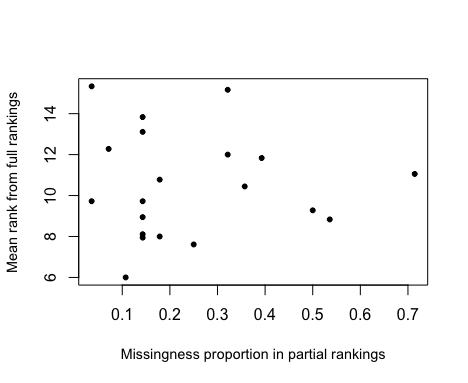
\includegraphics[width=0.65\textwidth]{figures/RJ2025_paper_scatter_beers.png}
      \caption{Relationship between the missingness proportion of the items in the partial rankings and their mean ranks from full rankings for the reduced \code{ranks\_beers} dataset.}
     \label{fig:scat_beers}
\end{figure}
%
The scatterplot in the Figure \ref{fig:scat_beers} does not reveal a clear association pattern. To formally assess this, we performed a rank-correlation test\footnote{We opted for the permutation test based on the Spearman correlation, as it is nonparametric and allows to better captures monotonic relationships in the case of small samples and ties occurring after rank-transformation.
} as follows
\begin{example*}
R> library(coin)
R> test\_df=data.frame(NaProp=na\_prop\_part\_by\_item, AvgRank=descr\_full\$mean\_rank)
R> perm\_test <- spearman\_test(AvgRank ~ NaProp, data = test\_df,
                             distribution = approximate(nresample = 10000))
R> perm\_test
	Approximative Spearman Correlation Test
data:  AvgRank by NaProp
Z = -0.18296, p-value = 0.8603
alternative hypothesis: true rho is not equal to 0
\end{example*}
The resulting $p$-value is well above the conventional 0.05 threshold, indicating no statistically significant evidence against
%of a relationship
%between the missingness pattern and the ranks observed in the full dataset, which is consistent with
the MAR assumption.
